% FIRST OF ALL:
% If you are using X-based Emacs to read this file, please switch on
% Syntax Highlighting by typing:
%    ALT-X  font-lock-mode   (or META-X on X-Terminals)
%
% That should make these comments nice and red so they can be easily
% distinguished from the actual code. 
% =======================================================================

% This is a template for  Masters' Theses at WPI.
% It complies (more or less) to the standards given by the Library 
% (as of February 1999)
%
% Feel free to use this file, but I give no guarantee for its compliance
% to standards (meaning I won't pay for the paper if the library rejects it :))
%
%
% The lengths (textheight, width etc.) are fine-tuned for ps1, ps2, and ps3, 
% but seem to be somewhat dependent on the machine you are using to compile, 
% the date, time, moon phase, the weather, and other quantum effects.
% You may have to change \oddsidemargin a little, but it's about 98% correct.
%
% Also, the spacing is correct (doublespacing with footnotes correctly
% singlespaced). Curiously, the font size is not specified in the
% regulations. So feel free to change it, but the majority of theses
% that I have seen is written in 12 point font.
% 
% As for the inclusion of graphics, I recommend the methods specified
% in ``latexguide.ps'' off the CS-GSO Website. You can use other
% methods including copy and paste with a photocopier, but I think
% using the graphicx package is the easiest.
%
% Have fun and good luck with the thesis.
%
%
%  Andreas Koeller (koeller@wpi.edu)
%
%
%

% The preamble
%
%
% 12 point font, and your thesis is a ``report'' to LaTeX
\documentclass[12pt]{report}

% this enables correct linespacing and graphics inclusion via 
%``\includegraphics''
\usepackage{setspace}
\usepackage{graphicx}
\usepackage{cite}
\usepackage{gensymb}


% leave 1.5in margin to the left and 1in margin to the other
% sides. Don't print page number in the margin (but rather above it)
\setlength{\textheight}{8.63in}
\setlength{\textwidth}{5.9in}
\setlength{\topmargin}{-0.2in}
\setlength{\oddsidemargin}{0.3in}
\setlength{\evensidemargin}{0.3in}
\setlength{\headsep}{0.0in}

% Start to write
\begin{document}
	
	% First things first: The Titlepage
	% This is the recommended format by the library
	%
	
	
	% Define \brk as a command for leaving a little vertical space. Makes
	% the titlepage easier to read - normally, this is NOT GOOD LATEX
	% STYLE!!!
	%
	\newcommand{\brk}{\vspace*{0.18in}}
	
	% No page number on the title page
	\thispagestyle{empty}
	
	% Center the whole title page
	\begin{center}
		
		\brk
		
		% Large font and bold face for the headline. Try to keep it at one or
		% two lines. Headlines over two lines will mess up the spacing, and you have to
		% manually finetune it. Note that the line break in the SOURCE CODE
		% does not affect the line breaking in the output file. If you want
		% hardcoded line breaks, you have to mark them with a double backslash (\\)
		
		{\large 
			\textbf{
				Aerial Software Defined Radio
			}
		}
		
		
		\brk
		by
		
		\brk
		Narut Akadejdechapanich\\Scott Iwanicki\\Max Li\\Kyle Piette\\Jonas Rogers
		
		% All this is constant:
		\brk\brk
		A Major Qualifying Project
		
		\brk
		Submitted to the Faculty of the 
		
		\brk
		WORCESTER POLYTECHNIC INSTITUTE
		
		\brk
		In partial fulfillment of the requirements for the
		
		\brk
		Degree of Bachelor of Science
		
		\brk
		in
		
		\brk
		Electrical and Computer Engineering
		
		\brk
		by
		
		\brk\brk
		\rule{3in}{1.2pt}
		
		\brk
		December 2016
		
	\end{center}
	
	
	\vfill
	APPROVED:
	
	\vspace{0.5in}
	\rule{3in}{0.8pt}
	
	Professor Alex Wyglinski, Major MQP Advisor
	
	\vspace{0.5in}
	\rule{3in}{0.8pt}
	
	Professor Yehia Massoud, Head of Department	
	
	
	% end of titlepage
	\newpage
	
	% This is the command for doublespacing when you use the setspace
	% package
	% Please do NOT use \baselinestretch, this will mess up everything,
	% cause earthquakes, tornados and lots of questions for me...
	% If you need a singlespaced paragraph (BAD STYLE!!!), use
	% \singlespacing or \onehalfspacing and enclose it together with the
	% paragraph in braces {\singlespacing This is my text... blah blah blah}
	%
	\doublespacing
	
	% Now you can start to be creative.
	% First, you need an abstract.
	% Fortunately, LaTeX has thought of that, so it's very easy:
	%
	\begin{abstract}
		This paper is the most important paper I have ever written. Therefore,
		everyone should read it, like it, and recommend it to all his friends.
	\end{abstract}
	
	% From here on, we need Roman page numbers according to the library
	% regulations. So let's assign those.
	
	\pagenumbering{roman} % or {Roman} if you like them capitalized
	
	% The next thing is the Preface (``Acknowledgements'').
	% No standard environment for that, so we'll format it by hand.
	%
	\begin{center}
		\textbf{Acknowledgements}
	\end{center}
	
	I would like to express my gratitude to my advisor who made
	sure the thesis has at least 120 pages, 200 pictures and lots
	of formulae and thus made me master \LaTeX{} like my native
	language.
	
	My thanks are also due to my reader... who has read the thesis
	in the two days that I gave him since it wasn't done until two
	days before due date.
	
	Thanks also to ... lots of friends, the fact that a week has
	seven days instead of only five as I had always thought, and
	the fact that I own a key to the building so I can work at four
	in the morning whenever I feel like it. That is, all the time.
	
	\clearpage
	
	% Automagic
	\tableofcontents
	
	% This will catch all objects enclosed in \begin{figure}\end{figure}
	% statements.
	\listoffigures
	
	% This will catch all objects enclosed in \begin{table}\end{table}
	% statements.
	\listoftables
	
	% And we need a clear separation between preface and text, otherwise
	% the numbering gets confused.
	\clearpage
	\pagenumbering{arabic}
	\setcounter{page}{1}
	
	\chapter{Introduction}

\section{Motivation}
Wireless signal localization can be used in many areas from surveillance to search and rescue. In the past, these efforts have been focused largely on visual inspection. Increasingly, research has turned to using wireless signal localization to provide non line-of-sight solutions.There are two major areas of research: the use of mass communication to inform people, and the use of new technologies to physically find people. PROBABLY SAY SOMETHING HERE ABOUT HOW WE’RE NOT REALLY DOING ANYTHING ABOUT INFORMING. There are new technologies emerging that are opening up new avenues for the location of people, namely low-cost, easy to use, highly maneuverable drones and cheap, powerful software defined radios (or SDRs).
Drones and SDRs have very similar advantages in their respective industries – high flexibility and maneuverability at low costs – so the combination of them is complementaryis a logical match. The motivation for this project is to integrate these technologies together to further enhance the state of the art in search, especially in areas with low visibility. Enabling a search of wireless signals opens the opportunity to locate sources otherwise impossible to locate. One such scenario would be a hiker lost in the Sierra Nevada forest with a cell phone, but no cell signal. Such a hiker would be nearly impossible to find visibly from a helicopter over the forest, but a drone with an SDR would be able to listen to beacons from their cell phone and calculate an approximation of their location. Another example scenario is the issue of locating the controller of a non-cooperative drone. Visually, this would be very difficult, but being able to sense the controlling signal and locate the controller would be possible through the use of an SDR.
\section{Current State of the Art}
The advent of small, highly maneuverable drones has allowed the expansion of search capabilities to a more fine scale with the use of mounted cameras. Low cost drones are also beginning to replace helicopters for traditional search and rescue missions [http://www.sciencedirect.com/science/article/pii/S0262407910617277]. The increased maneuverability and decreased cost is driving the movement toward drones.
Another quickly growing technology is the Software Defined Radio, which allows for easy reconfiguration. This allows an SDR to receive and transmit a wide range of waveforms. Using SDRs, it’s possible to create an intelligent radio that can modify its own parameters to best match its environment \cite{int_radio}. SDRs have also been used in a passive listening configuration to create a radar receiver {http://ieeexplore.ieee.org/document/5960663/}. The amount of flexibility these radios provide over traditional hardware radios is perfect for any application that will benefit from tuning to different frequencies, bandwidths, and modulation schemes.
Research in physically finding subjects has produced some novel ideas using these new technologies. In a paper published in 2010, researchers note that more and more people have their cell phone on their person at all times. They investigate the detection of these phones by their wireless transmissions {http://ieeexplore.ieee.org/document/5647107/}. In another research paper, the use of SDR hardware as a radar was investigated. Through the programmability of the SDR, the researcher was able to transmit and receive radar pulses with proper time and phase coherence, properties necessary to function as a radar receiver {https://etd.ohiolink.edu/!etd.send_file?accession=wright1176142845&disposition=attachment}. There is no mention in the published literature, however, of combining SDR technology with drone technology.
\section{Proposed Design and Contributions}
The goal of this project is to assess and demonstrate the utility of an aerially maneuverable SDR by integrating a commercially available SDR with a low cost aerial drone. By taking advantage of a drone's maneuverability, a multitude of new sampling positions are reachable, resulting in higher accuracy for locating signal sources.
The design consists of a lightweight SDR connected to a loosely directional multi-frequency RF front-end. The directionality of the antenna provides the opportunity for more accurate measurements: instead of simply measuring the signal strength at multiple points to triangulate, the platform will be able to identify the strength and origin direction, reducing the number of points needed for, and therefore speeding up, the localization of a signal source. therefore speeding up the process. Managing the SDR and sample processing is a single board computer (SBC), chosen for its balance between low weight, low power consumption, and ample processing power. In order to maintainMaintaining usabilityneutrality between different drone platforms, the platform will not explicitly communicate with its carrier drone, and will therefore include its own GPS receiver and other orientation sensors. This platform will be henceforth referred to as the Modular Aerial Software Defined Radio (MASDR) platform. <I think we should have a system diagram, idk whether here or later on, but somewhere>
This project adds to the state of the art by performing research into the combination of these two newly developed technologies. The findings from this project will provide new knowledge on the ability to localize wireless signals using an aerially mounted software defined radio. Creating this MASDR platform will open the door to many more discoveries and products through further more research and development. With more time to spend on software development, the MASDR platform would become much more capable in all aspects.
In addition to adding to the state of the art, this project seeks to develop a multipurpose platform which can be used for further research into the wireless spectrum from any location in the airspace. This could be used for channel modeling, <someone help i don’t know enough buzzwords>, and many more experiments into the behavior of various wireless signals in various environments.
\section{Report Organization}
This report is organized into seven chapters, the Introduction, Background, Proposed Approach, Methodology, Implementation, Results, and Conclusions. The Introduction presents the motivation for the project and the current state of the art to provide context for how this project relates to other prior and ongoing research. The Background chapter provides information on technologies and techniques used to make decisions and complete this project. In the Proposed Approach chapter, the report outlines the decision-making thought process for technical planning of the project. The Methodology chapter lays out the detailed plans of the project, its components, and the tests to verify functionality. The Methodology is followed by the Implementation chapter, which describes the implementation of the project in terms of hardware, software, and communications. In the Results chapter, the findings are presented organized by the test each finding came from. Finally, the Conclusions chapter summarizes the findings and provides recommendations for future work in the area.
	\chapter{Digital Communications and Spectrum Sensing Overview}
This chapter will introduce various fundamental topics that were taken into consideration in the design of the aerial software defined radio platform developed in this MQP. The topics proposed include spectrum allocation, energy detection, wireless transmitter localization, software defined radio, and aerial flight platform.

\section{Spectrum}
Wireless communications are transmitted through the use of the electromagnetic spectrum. The spectrum consists of a multitude of frequency bands that have been allocated for specific uses.

\subsection{Spectrum Usage}
The spectrum of radio frequencies used for wireless communications is managed by the government to promote efficient use and net social benefit. The National Telecommunications and Information Administration (NTIA) and the Federal Communications Commission (FCC) regulates the allocation of these frequencies in the United States as shown in Figure \ref{fig:freq_chart} \cite{FCC_Info}. 
\begin{figure}[ht]
\centering
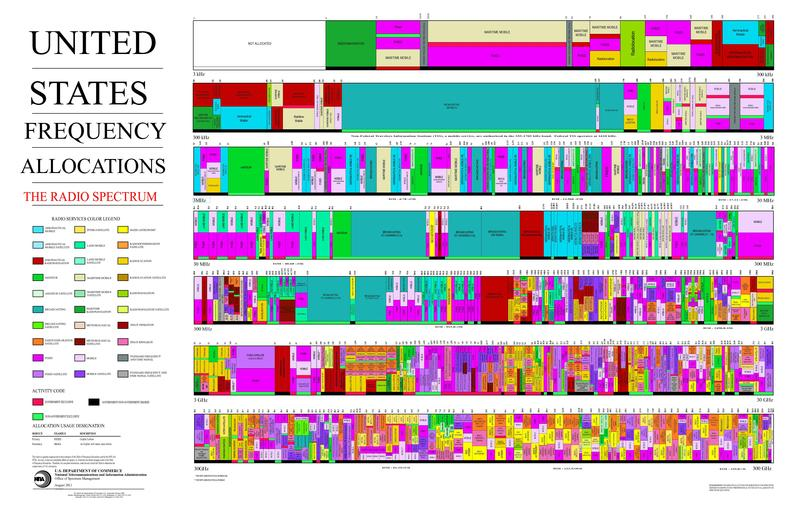
\includegraphics[width=0.70\textwidth]{img/the_radio_spectrum.jpg}
\caption{United States Frequency Allocation Chart \cite{FCC_Info}}
\label{fig:freq_chart}
\end{figure}
As seen from the figure, the spectrum is divided into smaller chunks where only specified entities can utilize legally. The usage of each chunk is determined by whether the NTIA and FCC require a license to use the band or not. Only operators with a license from the government can operate in the licensed bands, with uses that include AM broadcasting, FM broadcasting, and cellular communication. However, unlicensed bands are open to any entity that wants to utilize them, but they must still follow certain guidelines for usage. Technologies that use unlicensed bands include microwave, bluetooth, and WiFi. \textbf{Maybe talk about the history of this a little, why it's split up like this and why the certain bands were unlicensed}

\subsection{WiFi}
WiFi first came about in 1985, when the FCC decided to open up several bands of wireless spectrum for use without a government license. In the early 1990s, the Institute of Electrical and Electronics Engineers (IEEE) realized that wireless communications needed to be standardized. A committee was formed that focused on providing a reliable, fast and robust wireless solution that would be able to scale for years to come. Therefore, the IEEE made an addition to its 802 standard which is used for local area networks, and thus the 802.11 standard was created in order to assure these things. Since then, there has been multiple iterations of the standard, and five sub-standards have been established for wireless communications called:802.11a, 802.11b, 802.11g, 802.11n, and 802.11ac. \cite{bergieee}

The first creation of the standard was 802.11 which was origionally created in 1997. The data rate was capped at 2 Mbps and transmitters transmitted on a frequency from 2.4 to 2.483 GHz. These transmitters used time-division duplexing which allows them to send uplink and downlink wireless traffic on the same RF channel. The transmitters also use interference mitigation techniques such as DSSS and FHSS which are protocols that switch wireless channels when there is other wireless interference present on that channel.

In addition to this, all the wireless standards also use a media access layer which is also known as the MAC layer.  This layer is used to assist the transmission by providing frame synchronization, and ecrypyion.  802.11 uses ecryption by using Wired Equivalent Privacy or WEP.  WEP consists of a 40 bit key that is used in order to access communication with a Wi-Fi transceiver.

WEP encryption, dynamic frequency selection, and the OFDM preamble are all have all been carried on from one standard to the next.  However, WiFi traffic can be transmitted using a variety of bandwidths dependant on their respective 802.11 standard.  Wi-Fi traffic can transmit using a 20 MHz, 40 MHz or 80 MHz bandwidth dependant on their 802.11 standard. 
\begin{table}[ht]
\centering
\caption{WiFi Protocols.  This table outlines the bandwidth, frequency spectrum and modulation type of each corresponding 802.11 interface. As the wifi protocols become newer from starting with 802.11a and ending with 802.11ac as the most recent, the protocols utilize wider bandwidths for communication, and offer a range of operating frequencies. MIMO-OFDM was also developed for later 802.11 protocols such as 802.11n and 802.11ac in order to support multipath propagation.}
\label{table:wifi_protocols}
\begin{tabular}{|l|l|l|l|}
  \hline
  Interface & Bandwidth (MHz) & Frequency Spectrum (GHz) & Modulation \\ \hline
          802.11a &              20 &                  5 &       OFDM \\
          802.11b &              20 &                2.4 &       DSSS \\
          802.11g &              20 &                2.4 &       OFDM \\
          802.11n &          20, 40 &            2.4 / 5 &  MIMO-OFDM \\
         802.11ac &      20, 40, 80 &                  5 &  MIMO-OFDM \\ \hline
\end{tabular}
\end{table}\par
These transmissions can vary when it comes to the entire frames information. However, each standard has the same preamble that signifies the start of a transmission, and what central freuency the transmission is on.  For 802.11, a wifi transmission is concentrated in one or more 20 MHz wide wifi channels or bins. At the 2.4 GHz band, Wi-Fi is allocated throughput 11 wireless channels ranging from 1 to 11.  However, only 3 of these channels (1, 6, and 11) are used due to each channel only being 5 MHz wide.  Since transmissions on the 2.4 GHz band are 20 MHz wide, the utilized channels are spaced enough to mitigate co-channel interference. A photo of the allocated spectrum is shown below:

%Put in the 2.4 GHz photo

Also, for protocols 802.11a, 802.11n and 802.11 ac, they also use the 5 GHz frequency band which contains a range of 45 channels from 36 to 165 spanning spectrally from 5180 MHz to 5825 MHz.  This allocation is shown below:

%include photo of 5GHz band

What first signifies a transmission on any of these wifi channels is the detection of the OFDM PLCP preamble which signifies which channel the information is being transmitted on. This preamble consists of  In addition to the preamble, you could also decode the information from the Data fields, however, all of that data is usually encrypted so that it prevents any unauthorized user from accessing it. \cite{wifi_book}

\subsubsection{MAVLink}
The Micro Aerial Vehicle Link (MAVLink) protocol is a free open source wireless communication protocol for controlling small unmanned aerial vehicles. This protocol first came about in 2009 by Lorenz Meier under LGPL license. \cite{MAVLINK_Website}  This protocol was designed to be a lightweight, header-only message marshaling library.  MAVLINK was first most commonly used with autopiloting software, but is trying to become the worldwide standard in drone communication. This communication protocol consists of communication with a slave drone and a master ground controller.  MAVlink controllers most commonly transmit data on the 2.4 GHz band along-side 802.11 wireless communications. Therefore, an airbourne receiver must be able to classify what type of signal it has received. To classify a MAVLink transmission, this can be done by demodulating MAVLink's GFSK modulated data, and decoding its data frame. 
\begin{figure}[ht]
\centering
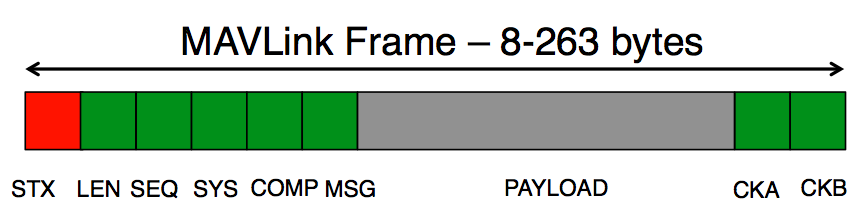
\includegraphics[width=0.70\textwidth]{img/mavlink-packet.png}
\caption{MAVLink Transmission Frame. The red STX frame signifies the start of a transmission. This frame will always be an 8 bit code of 0xFE used for start of frame detection. The following parameters give information about the payload such as it's size and who the data was meant for.  The payload category is a data field which contains a library-based command for the drone to perform.}
\label{fig:MAVlink_frame}
\end{figure}\par
\begin{table}[ht]
\centering
\begin{tabular}{|l|l|l|l|}
  \hline
  Byte Index & Content & Value &  Purpose \\ \hline
          0 &	Packet start sign &                  0xFE &       Indicates start of a new packet\\
          1 &   Payload length &                0 - 255 &       Indicates length of the following payload \\
          2 &   Packet Sequence &               0 - 255 &       Enables packet loss detection because each component counts up its send sequence \\
          3 &   System ID &            1 - 225 &  Identifies the sending system; enables multiple platforms to use the same network \\
          4 &   Component ID &         0 - 255 &  Identifies the sending component; allows for multiple components on the same platform \\
          5 &	Message ID &		   0 - 255 &  Identifies the message being sent defines the payload and how it should be decoded \\
          6 - n+6 &	Data & 			   0 - 255 & Data of the mesasge depends on message ID \\
          n+7-n+8 & Checksum & & ITU hash of bytes including MAVLINK parameter computed from message fields to prevent decoding from a different protocol version \\ \hline
\end{tabular}\end{table}
\par
Also, opposed to wifi signals, MAVLink transmissions are all non-encrypted, making it vulnerable to things such as network attacks or an unauthorized user operating the drone. Any user can send signals to a drone using a GFSK transmitter and the drone has no knowledge on who the correct user \cite{mavlink_vuln}.

\subsection{GPS \textbf{Needs more content}}
Global Positioning System, or GPS, provides highly accurate location information to a user with a receiver module. This technology was developed during the height of the cold war in the 1960s \cite{gps_info}. GPS works by using a network of 24 satellites that are transmitting on 1575.42Mhz using a division coding scheme. The individual satellites send out information such as the current system time, and their locations. Given the locations of the satellites, as well as the calculated time of travel from the satellites to the receiver, the GPS receiver then performs localization based on this received information. The accurate time stamping required to perform this localization is only possible because each GPS satellite is capable of maintaining a highly accurate clock, and each receiver determines its current time through the interpretation of satellite data. This accurate clock information is used for the synchronization of clocks across cellular telephone systems, and other time critical applications \cite{GPS_Book}.

\section{Spectrum Sensing}
As described in the previous section, the electromagnetic radio spectrum is becoming increasingly crowded, with this issue only accelerating as the Internet of Things becomes more widespread \cite{sensing_iot}. With the conventional approach of spectrum management, users are assigned a specific frequency band. This method becomes less sustainable with the increasing number of users, especially in the unlicensed frequency bands. In order to combat this, Cognitive Radio (or CR) was created to utilize spectrum more efficiently \cite{wyglinski_book}. Cognitive radios are designed to provide a highly reliable connections for all users of the network, by sensing what frequencies are being used at any given moment, and utilizing the unused parts of the spectrum. The types of signals to be sensed are divided into two different groups: uncooperative users and cooperative users \cite{spectrum_sense_methods}. \par
The process of spectrum sensing is made more complicated by uncertainties in the received data, including channel uncertainty and noise uncertainty. With channel uncertainty, the received signal strength can fluctuate based on characteristics of the channel, such as channel fading or shadowing. Noise uncertainty refers to the fact that the power of the noise is unknown to the receiver, making it difficult to achieve a specific sensitivity \cite{spectrum_sense_methods}. In order to have a functioning CR, both uncertainties need to be addressed. \par
As the types of signals to be sensed are split into non-cooperative and cooperative systems, so too are the methods of sensing. The present MQP involves passive sensing of the spectrum, where only the methods concerning the former will be discussed.

\subsection{Energy Detection}
The simplest method of non-cooperative sensing is energy detection. In this approach, the power spectral density (or PSD) of the received signal is taken\cite{sensing_energy}. The PSD represents the measure of a signal’s intensity in the frequency domain computed through the fast fourier transform of a signal. This is then bandpass filtered to contain only the frequency bands being watched. These frequency bands are then integrated, to determine how much energy is present in the band. If this passes a certain threshold, the frequency band is marked as occupied. A MATLAB example of Energy Detection is provided in Appendix \ref{app:energy_detection}, and a flow diagram of Energy detection is shown in Figure \ref{fig:energy_detection}.
\begin{figure}[ht]
\centering
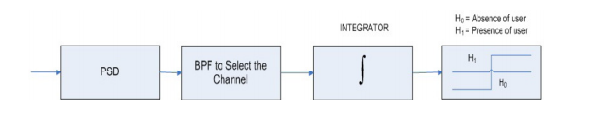
\includegraphics[width=0.70\textwidth]{img/energy_detection.png}
\caption{Flow diagram of energy detection.}
\label{fig:energy_detection}
\end{figure}\par

This method of detection is the most simple as it does not require information about the signal ignoring key aspects of signals such as modulation method and pulse shaping. Because of this, it is the simplest detection method to implement. However, an assumption made in using energy detection is that the signals being searched for have significantly more power than the noise and interference of the channel. This does not always prove to be true. In addition to this, energy detection cannot be used to distinguish signals using the frequencies measured, as no pulse shape information is determined.

\subsection{Matched Filter}
Another approach to spectrum sensing is through the use of matched filters. Matched filters are designed to maximize the signal to noise ratio (SNR) given an input signal, which we will call $s_{in}$ \cite{sensing_energy}. To sense signals through matched filtering, prior knowledge of the reference signal (or $s_{ref}$) to be detected must be known. The $s_{in}$ will then be correlated with $s_{ref}$. This produces a value m, that will be compared to a threshold value. This process is described in Equation \ref{eq:matched} below and in Figure \ref{figure:matched_filter}
. N represents the length of the reference signal, in samples. 
\begin{align} \label{eq:matched}
    m &= \sum_{k = 0}^{N}s_{in}[t-k]s_ref[N-k] 
\end{align}
\begin{figure}[ht]
\centering
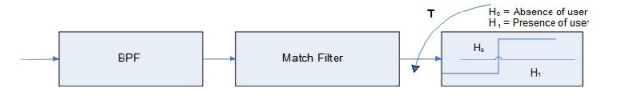
\includegraphics[width=0.70\textwidth]{img/match_filter.png}
\caption{Flow Diagram of matched filter. WORDS}
\label{figure:matched_filter}
\end{figure}\par
Matched filters rely on prior knowledge of the characteristics of signals to be detected, otherwise this method will not be accurate. The prior knowledge constraint limits the use of signal detection when unexpected signals are involved. Furthermore, matched filter detection is optimal with stationary gaussian noise to hinder distortion. This will limit the real world applications for signal detection with matched filtering as most channels are time-varying and non-gaussian \cite{channel_fade}. A MATLAB example of Energy Detection is provided in Appendix \ref{app:matched_filter}.

\subsection{Cyclostationary Feature Detection} \label{Cyclostationary Feature Detection}
Cyclostationary Feature Detection (or CFD) depends on the fact that all communication schemes have some sort of signal repetition as a core aspect. A signal with this kind of repetition is called a Cyclostationary Process\cite{cyclostat_journal}. Because of this property, when you correlate the signal with itself (or autocorrelation), there will be repeated peaks. The periodic nature of the signal also means that the autocorrelation will be periodic as well. This allows it to be expressed as a Fourier Series, called the Cyclic Autocorrelation Function (CAF) and denoted by $R_x^\alpha(\tau)$\cite{cyclostat_text}.\par 

\begin{align}\label{eq:caf}
    R_x^{\alpha(\tau)} &= lim(t->\infty) \frac{1}{T} \int_{-T/2}^{T/2} R_x(t,\tau)exp(-j2\pi\alpha t dt)
\end{align}

Where $R_x(t,\tau)$ is the autocorrelation function of x at t with x at $\tau$. This function gives us an understanding of the times when the signal repeats, but is missing vital information of the repeated frequencies. By taking the fourier transform of $R_x^\alpha(\tau)$, we can get a better understanding of the frequencies in the Cyclostationary Process. This is denoted as $S_x^\alpha(f)$, and is equal to \cite{cyclostat_text}:  \par

\begin{align}\label{eq:scf}
S_x^\alpha(f)=\int_{-\infty}^{\infty} R_x^\alpha(\tau)exp(-j2\pi f\tau d\tau) 
\end{align}
\par

This is called the Spectral Correlation Function (SCF). When it is normalized, it becomes the Spectral Coherence Function (SOF) \cite{cyclostat_text}:
\begin{align}\label{eq:caf}
C_x^\alpha(f) = \frac{ S_x^\alpha(f)}{ (S_x^\alpha(f+\alpha/2) S_x^\alpha(f-\alpha/2))^{1/2}}
\end{align}\par
The SOF is from between 0 and 1, and represents the strength of the periodicity at that point. By plotting this value, the unique response of the Cyclostationary Process can be found, allowing for it to be categorized.\par

One of the major benefits of CFD is that it is not nearly as affected by noise. Under the generally held assumption that noise is white and Gaussian, there is no periodic response, and as such noise is not factored into CFD. Example plots from an implementation of CFD are shown below. \par
% \begin{figure}[ht!]
% \subfloat{
% 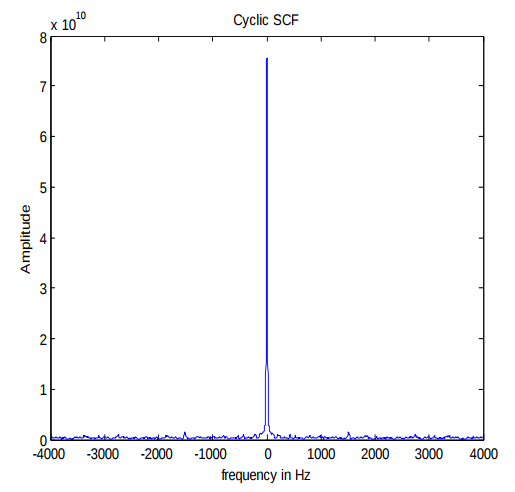
\includegraphics{img/cyclic_scf.png}
% \caption{cyclic scf \textbf{Needs to be 2-3 sentences -Narut}}
% \label{fig:cyclic_scf}
% }

% % \begin{subfigure}{0.5\textwidth}
% % 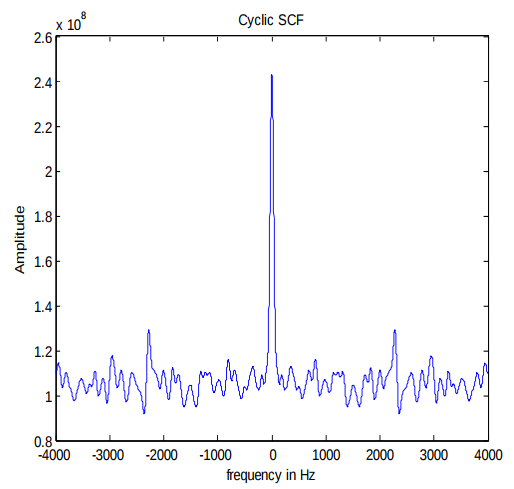
\includegraphics[scale=0.4]{img/cyclic_scf_bpsk.png}
% % \caption{cyclic scf BPSK \textbf{Needs to be 2-3 sentences -Narut}}
% % \label{fig:cyclic_scf_bpsk}
% %\end{subfloat}
% \end{figure}
% % \begin{figure}[ht]
% \centering
% 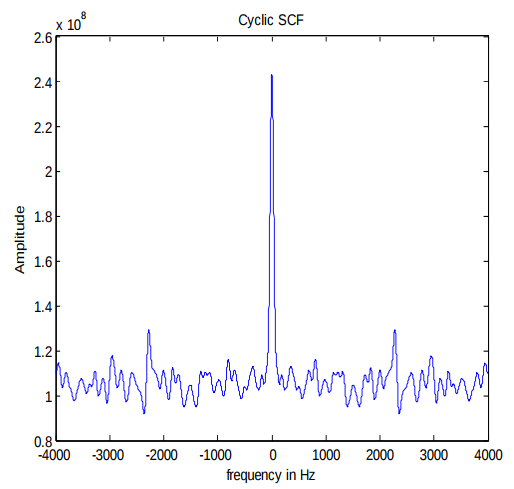
\includegraphics[scale=0.4]{img/cyclic_scf_bpsk.png}
% \caption{cyclic scf BPSK \textbf{Needs to be 2-3 sentences -Narut}}
% \label{fig:cyclic_scf_bpsk}
% \end{figure}
% \begin{figure}[ht]
% \centering
% 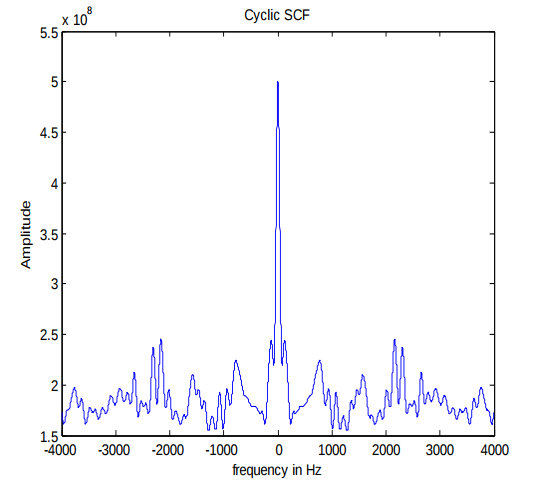
\includegraphics[scale=0.4]{img/cyclic_scf_qpsk.png}
% \caption{cyclic scf QPSK \textbf{Needs to be 2-3 sentences -Narut}}
% \label{fig:cyclic_scf_qpsk}
% \end{figure}

The primary downside to Cyclostationary Feature Detection is the complexity and time required to properly utilize it. The complexity lies in the number of integrals and correlations that need to be computed in order to implement CFD. In addition, the system needs to listen for signal long enough for the Cyclostationary Process to repeat. Because of these downsides, it is not common to be used on embedded systems. \par


\section{Radio Localization}
Once a signal has been identified on a measured frequency, the next step is localization. Localization refers to the act of determining the location of a transmitted signal \cite{local_conf}. There are many different methods for localization. However, many of them become impractical for mobile passive sensing. In the following section, a variety of localization techniques will be discussed, as well as the practicality of implementing each of them.\par
For each of the techniques discussed below, the same basic concept is used. Three different receivers are placed around the transmitter being located, as shown in Figure \ref{fig:node_localization}.  They will be called stationary nodes and the unknown node, respectively. Each stationary node gets information about its location relative to the unknown node simultaneously. For Time Difference of Arrival (TDoA), Time of Arrival (ToA), and Received Signal Strength (RSS) Localization, each stationary node calculates the distance to the unknown node. This information is used with the known locations of the stationary nodes to localize the unknown node. Angle of Arrival (AoA) functions differently and will be described in a separate section. \par

%12/5/16 A Page break should go here, assuming nothing changes. Max
\begin{figure}[ht]
\centering
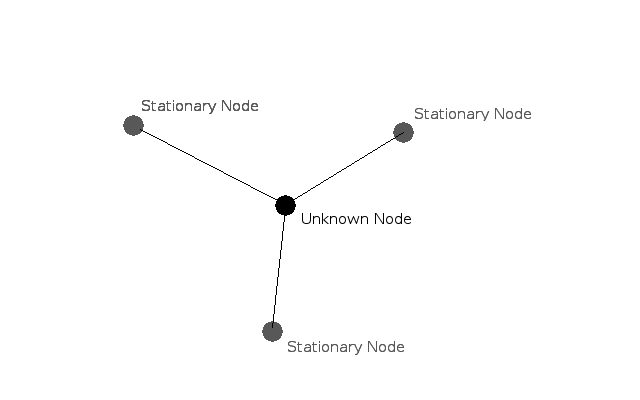
\includegraphics[scale=0.5]{img/node-localization-lines.png}
\caption{Node Localization \textbf{Needs 2-3 sentences and needs to be drawn more realistically w/ buildings and such -Narut}}
\label{fig:node_localization}
\end{figure}\par

Table \ref{table:local_methods} shows the most important details of the localization techniques that will be described. \par
\begin{table}[ht]
\centering
\caption{Localization Methods}
\label{table:local_methods}
\begin{tabular}{|l|l|l|l|}
    \hline
  Localization Method   & Mathematical Technique    & Needs Unknown Node Participation? & \\ \hline
         TDoA           & Distance                  & Yes                               & \\
          ToA           & Distance                  & Yes                               & \\
          RSS           & Distance                  & No                                & \\
          AoA           & Angle                     & No                                & \\
    \hline
\end{tabular}
\end{table}\par

%%%%%%%%%%%%%%%%%%%%%%%%%%%%%%%%% got here -Narut
In the distance-based localization techniques, each stationary node knows the unknown node is a certain distance away \cite{local_conf}, allowing for it to be anywhere along a circle, with the stationary node in the center. By finding out where all three circles intersect, the unknown node can be located. The distance of the unknown node from any of the stationary nodes is calculated using Equation \ref{eq:dist_coord}.\par 
\begin{align}\label{eq:dist_coord}
D_i &=\sqrt{(X - x_i)^2 + (Y-y_i)^2}
\end{align}\par
By plugging in the locations and calculated distance for each stationary node, a system of equations is created, making it possible to solve for the location of the unknown node.\par
%TDoA
One method of localization is Timed Difference of Arrival (TDoA) \cite{local_conf}. In this method, the unknown node transmits a signal over radio frequencies. Using the difference in the timestamp and actual time of receiving the signal, the stationary nodes can calculate the distance between each stationary node and the unknown node, using Equation \ref{eq:dist_light}. c represents the speed of light.
\begin{align}\label{eq:dist_light} 
    d &= c*(t_{actual} - t_{expected}) 
\end{align} \par
This method of localization is dependent on three things: the synchronization of the nodes involved, the participation of the unknown node, and the existence of three or more stationary nodes. In the use case presented by this MQP, the most difficult part about this implementation is the participation of the unknown node. Since the aerial platform has no communication with the object being localized, this method is impractical. \par

%%Time of Arrival
Using the Time of Arrival (or ToA) approach is similar to TDoA in concept \cite{local_conf}. Each of the stationary nodes sends a signal at a specific time, known to the unknown node, $t_0$. Using the difference in $t_0$ and the time that the base receives the signal, or $t_1$, the unknown node calculates the time the signal was in the air, and uses the speed of an electromagnetic wave to determine the distance to the stationary node, as described above. With three of these calculations, the location of the unknown node can be triangulated.\par

Like TDoA, ToA requires the synchronization of the nodes involved \cite{local_conf}. In most implementations, this is done using digital timestamps. It also requires the participation of the unknown node. Similarly to TDoA, these requirements make ToA an impractical fit for this MQP. \par

%RSSi Localization
Unlike the previous two methods, which depend on knowing the time a signal was sent, received signal strength localization uses the strength of a received signal to localize the unknown node \cite{local_conf}. Each of the stationary nodes receives the signal being output by the unknown node. Using the Equation \ref{eq:rssi} and Equation\ref{eq:rssi_dist}, the stationary nodes can calculate the distance to the unknown node \cite{rss_calc}. From this, they can triangulate the location as described before.\par
\begin{align}
\label{eq:rssi} RSSI &= 10\alpha log(d) \\ 
\label{eq:rssi_dist} d &= 10^{(RSSI-RSSI_{calibration})(-10\alpha)} + d_{calibration}
\end{align}
\par
Because RSSI localization depends on the measurement of the signal strength, it is adversely affected by sources of noise and interference, like channel fading and multipath interference \cite{local_conf}. This makes the technique have lower accuracy. The effects of noise and shifting channels can be somewhat mitigated by averaging the RSS data.

%Angle of Arrival.
\textbf{MATLAB EXAMPLE OF AoA probably needed}
Unlike the previously described methods, some localization techniques use the angle that the signal arrives at relative to a reference direction, or the Angle of Arrival (AoA) \cite{local_aoa}. To use this method, antenna arrays or directional antennas are used to determine the angle at which the signal arrived at. Similarly to TDoA, the stationary nodes wait for a signal from the unknown node. Using the directional antenna or the antenna array, the AoA is calculated at each stationary node. From each of these nodes, a ray can be drawn originating from the node that follows the angle of arrival. The unknown node is located based on where the rays intersect.

\begin{figure}[ht]
\centering
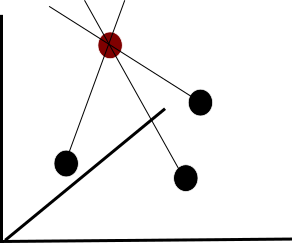
\includegraphics[scale=0.5]{img/path4188.png}
\caption{Angle of Arrival Diagram}
\label{fig:aoa_diagram}
\end{figure}\par
AoA localization consists of similar issues as other techniques. Noise and channel issues still come into effect. Additional issues occur if these unknowns can’t be dealt with. Another constraint is the requirement for highly directional sensing, which complicates the sensing of a signal before localizing it. This can either be done with many antennas or a very directional antenna, but it adds complexity.

\section{Software Defined Radio}
Due to the rapidly increasing number of users dependent on efficient spectrum allocation for communication, the use of reprogrammable radios has become an integral part of designing communication systems. Radios exist in a wide range of devices, such as cell phones, cars, televisions, garage door openers, and computers. A radio is any device that transmits or receives wireless signals that are within the radio frequency band of the electromagnetic spectrum. A software defined radio (SDR) is defined as a “radio in which some or all of the physical layer functions are software defined” \cite{sdr_forum}. Traditional hardware based radios are nearly impossible to modify post-production, and have limited ways to be repurposed. SDRs, on the other hand, are comparatively inexpensive, highly reusable, and are easily configurable to support multiple waveform standards.\par
There are multiple different families of SDRs, two of which are RTL and Universal Software Radio Peripheral (USRP). An RTL is a low cost SDR that uses a DVB-T TV tuner dongle based on the RTL2832U chip set \cite{rtl_sdr}. The DVB-T TV tuner was converted to be used as a wideband SDR using a new software driver. The RTL-SDR can be used for many applications including listening to aircraft traffic control, decoding ham radio packets, and sniffing GSM signals. The USRP is a flexible transceiver that is able to use a standard PC to prototype wireless systems. USRPs are able to prototype a wide range of single-channel and multi-input multi output (MIMO) wireless communication systems \cite{USRP_NI}. USRPs can be programmed using software frameworks including GNU Radio, Matlab, Simulink, LabVIEW, C++.\par
SDRs can be implemented on field programmable gate arrays (FPGA), digital signal processors (DSP), programmed System on Chips (SoC), general purpose processors (GPP), personal computers (PC), or other reprogrammable application specific integrated circuits (ASICs). The use of these reprogrammable technologies allows for the possibility of constant updates or dynamic radio systems without the need to add additional hardware. The primary goal of designing an SDR is to implement as much of the radio in the digital space, minimizing the use of analog components. The digital portion of an SDR performs the data compression, encoding, modulation, demodulation, decoding, and decompression in software. The only analog components are a digital to analog converter (DAC), an analog to digital converter (ADC), and a RF circuit. The RF circuitry on the transmitter consists of a smoothing filter to reduce the hard edges of the baseband signal that the DAC outputs as well as circuitry to upconvert the baseband signal. The RF circuitry on the receiver side consists of a downconverter to move the signal to the baseband as well as filters to remove noise from the signal. The DAC and ADC serve as the bridge between the analog and digital realms enabling the software defined signal to be converted to an analog one to transmit and receive, then converted back to digital on the receiving end shown below in Figure \ref{fig:sdr_flow_diagram}.
\begin{figure}[ht]
\centering
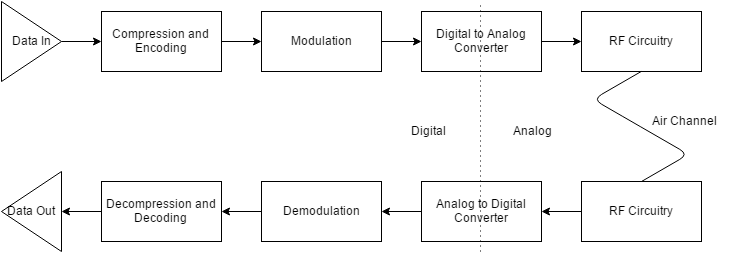
\includegraphics[width=0.70\textwidth]{img/sdr_diagram.png}
\caption{Flow diagram of an SDR with the distinction between the digital and analog components}
\label{fig:sdr_flow_diagram}
\end{figure}\par
A typical transmitter will pass a modulated signal to the DAC which will take the digital input and output a baseband analog signal. The analog signal will be upconverted to the carrier frequency in a single step or multiple steps. The receiver will take the received analog signal and downconvert it. It then passes the baseband analog signal to the ADC to convert the signal back into digital for the SDR to process. The capabilities of the ADC and DAC, such as the as the bandwidth and noise tolerance of these two components, will dictate the complexity the RF circuitry that is needed to satisfy these requirements.\par
A software defined radio, such as an adaptive radio, has the capability to be much more sophisticated than an analog counterpart. Adaptive radios are able to monitor their own performance and adjust their parameters to ensure the highest quality of service \cite{cog_radios}. A more advanced type of adaptive radio is the cognitive radio, mentioned in \ref{Cyclostationary Feature Detection}, which is able to monitor, sense, and detect conditions of their operating environment and adjust its characteristics to match those conditions. This allows the radio to provide improved performance and quality of service. These radios are able to find and transmit on open gaps in a radio spectrum. This allows for minimal interference from other sources. Cognitive radios use the trends of the channel to determine whether to switch channels or continue using the current channel. The most advanced type of adaptive radio is the intelligent radio. These radios are capable of machine learning which enables the radio to improve its algorithm for adjusting the radio's parameters based on previous experience when changes to performance or the environment occur \cite{int_radio}. The relationship between these types of radios is shown below in Figure \ref{fig:sdr_relationship_diagram}.\par
\begin{figure}[ht]
\centering
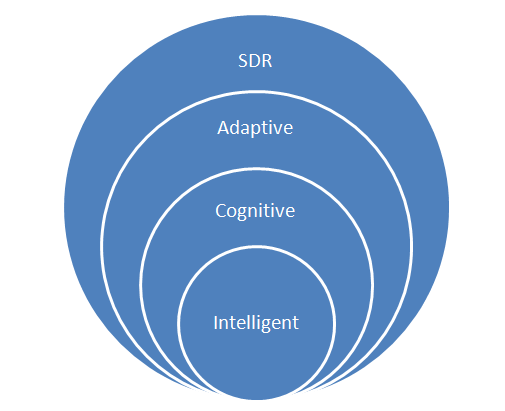
\includegraphics[width=0.70\textwidth]{img/sdr_diagram2.png}
\caption{The relationship between SDR, adaptive radio, cognitive radio, and intelligent radio}
\label{fig:sdr_relationship_diagram}
\end{figure}\par
There are three major groups of algorithms that intelligent radios are based on: machine learning, genetic algorithms, and fuzzy control \cite{amraoui2012intelligent}. A type of machine learning is the neural network. Neural networks are a large group of nodes that are used to solve problems similarly to how the human brain operates. When new information is aquired, this information is incorperated into the algoithim to be used to improve the output \cite{amini2011universal}. This technique is used to estimate the performances of WIFI networks and respond to changes in the network. Fuzzy logis is usually combined with neural netowrks that adapt to the envirnment during the operation of an intelligent radio. A fuzzy logic control system is used to find the solution to a problem given imperfect information \cite{amraoui2012intelligent}. There are three main components in a fuzzy logic controller: fuzzifier, fuzzy logic processor, and defuzzifier.The fuzzifier maps the inputs into fuzzy sets, the fuzzy logic processor determines a fuzzy output based on a set of rules, and the defuzzifier transforms the fuzzy output into a crisp output. One of the main advantages to fuzzy logic is its low complecity, which is extremely useful in real-time radio applications. Another example of an algorithm used in intelligent SDRs is the wireless system genetic algorithm (WSGA). This algorithm is a multi-objective genetic algorithm (MOGA) designed for the control of a radio by modeling the physical radio system as a biological organism and optimizing its performance through genetic and evolutanry processes \cite{rondeau2004cognitive}. Each aspect of the radio such as payload size, coding, encryption, and spreading can be considered gene that can be modified through these processes. These genes are combined into a chromosome that is used to evolve the system. The algorithm analyzes the effectiveness of the chomosome through weighted fitness functions defined by performance evaluations of the current radio channel \cite{rondeau2004cognitive}. 
\textbf{Write Conclusion}

\section{Aerial Platforms}
The inspiration behind this MQP was to discover how much information could be gathered from the wireless spectrum when observed from the air. Aerial platforms have been used in the past for surveying tasks like geographical mapping. \cite{geomap_patent} These systems generally use a camera to capture visual images from above. To facilitate flying our sensory system, three main mobile methods of elevating the sensory unit were considered: kites, fixed-wing aircraft, and multicopters, each of which will be described in detail below.

\subsection{Kites}
A kite is a passive structure tethered to the ground that stays airborne by catching wind \cite{kite_book}. There are many different styles of kite, including parafoil, rokkaku, delta, and sled, but they all rely on the same principle to fly \cite{kite_book} \cite{kite_iqp}. Kites have near unlimited flight time and high payload capacity when operated in favorable conditions, but in exchange they sacrifice control, reliability, and maneuverability.\par
Since kites are powered by the natural wind in the atmosphere, they do not require any power to stay aloft. However, depending on the style of kite, they do require specific conditions to fly. Almost all kites need at least 2-3 mph of wind to get up into the air, and delta and rokkaku are limited to a maximum of 12-16 mph \cite{kite_iqp}. Parafoils can fly in wind up to 20 mph, but can be unstable.\par
The only control a user has over a kite in flight is changing its height by letting out or reeling in more of the tether cord. Different styles of kite have different flying angles, which impacts the amount of weight they can carry. Some kites, such as the rokkaku and delta (example in Figure \ref{fig:delta_kite}) styles, can be modified during assembly to change their angle of flight, where higher angles produce more lift. While parafoils can inherently carry more weight, they also have a low flying angle, which can be problematic in some scenarios. The preparation for flight involves assembling the kite, normally by inserting cross-bars, and unreeling the tether in an open space that allows the kite to take off.\par
\begin{figure}[ht]
\centering
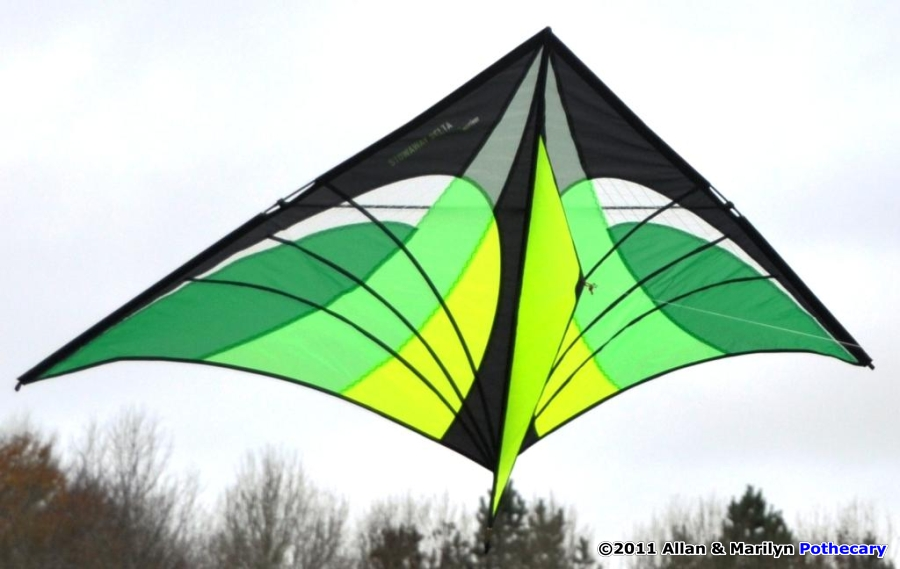
\includegraphics[width=0.70\textwidth]{img/delta-kite.jpg}
\caption{A delta style kite. Delta style kites can be configured to fly at high angles, allowing them to be flown in laterally constrained locations.}
\label{fig:delta_kite}
\end{figure}\par
Kites are, by necessity, constructed of very light materials and cannot support much extra weight in light wind situations. Again, the style of kite affects the carrying capacity: deltas can carry a moderate amount of weight, but need higher winds to stay aloft. Parafoil and rokkaku kites can carry more weight, with 10 lbs being on the low end.\par
One application of kites that concerns the carrying capacity is kite aerial photography, which consists of a camera mounted to a kite as a low-cost way to take aerial pictures. Varying flying conditions force photographers to mount cameras to many different types of kites with differing angles of flight, payload capacity, and stability. Advanced photographers also utilize mounting rigs to stabilize and sometimes rotate the cameras in flight \cite{kite_iqp}.\par
The pros and cons of a kite as a platform for the SDR system are enumerated in Table \ref{table:kite_pc}.
\begin{table}[ht]
\centering
\caption{Kite Pros and Cons}
\label{table:kite_pc}
\begin{tabular}{l|l}
  Pros & Cons \\ \hline
  cost & maneuverability \\
  flight time & deployment time \\
  payload capacity & \\
\end{tabular}
\end{table}\par

\subsection{Fixed-wing Aircraft}
A fixed-wing aircraft is a rigid structure with one or more rotors oriented forward that gains lift from the flow of air over its wings \cite{airplane_book}. A diagram showing this lift mechanism can be found in Figure \ref{fig:airfoil_lift}. This section will focus on radio controlled (RC) aircraft since they are the type being considered for use in this MQP. An RC aircraft’s movement is typically controlled by servos onboard that move flaps to change the surface of the aircraft, in turn changing the dynamics of flight and causing the plane to respond. RC aircraft are very efficient in terms of flight time to power used because the lift comes from the shape of the wings, not the speed of the motor \cite{airplane_site}. Since the lift comes from the wings, fixed-wing aircraft have a moderate flying time and can carry a moderate amount of weight, but the plane’s motion is very linear so its maneuverability is limited.\par
\begin{figure}[ht]
\centering
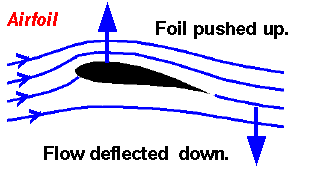
\includegraphics[width=0.70\textwidth]{img/airfoil_lift.png}
\caption{Airfoil lift generation. As air flows past the airfoil, it is forced downward, in return forcing the aircraft upward.}
\label{fig:airfoil_lift}
\end{figure}\par
The flight time of most battery powered RC fixed-wing aircraft is around half an hour assuming some aerobatics \cite{airplane_book}. In a surveying role, with the plane flying low circles, the flight time would likely increase slightly. There are also gasoline powered aircraft with small engines onboard to power the main propeller. Gasoline has a very high energy density, so it’s possible to fly for multiple hours with a gasoline powered aircraft.\par
Fixed-wing aircraft have a fairly lenient payload capacity. One thing to consider about adding payloads to fixed-wing aircraft is that since the aircraft’s flight is so heavily impacted by the body shape, any payload will need to be incorporated into the body of the aircraft to minimize airflow disturbance. To get more lift, and thus carry more weight, the plane simply needs to fly faster to force more air over the wings. This has drawbacks however, as spinning the propeller faster will drain the power source faster and decrease maneuverability.\par
Fixed-wing RC aircraft have been used in the past for similar tasks. In one example, a group of students at WPI developed a search and rescue platform using a fixed-wing RC aircraft \cite{airplane_iqp}. An example of a fixed-wing RC aircraft is shown in Figure \ref{fig:fixed_wing}.
\begin{figure}[ht]
\centering
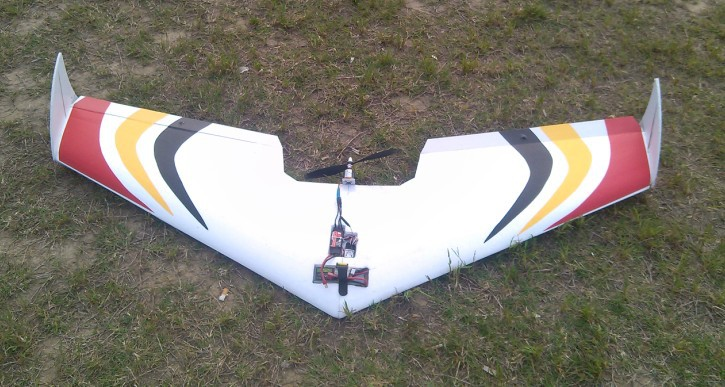
\includegraphics[width=0.70\textwidth]{img/fixed-wing.jpg}
\caption{A fixed-wing RC aircraft. This is a flying wing style craft with a rear propellor. Its flight would be greatly hindered by any protrution of a mounted system.}
\label{fig:fixed_wing}
\end{figure}\par
A fixed-wing aircraft is able to cover large distances flying laterally, but it is not able to stop mid-flight and hover in place \cite{airplane_book}. Its turning radius is often quite large, and it must not drop below a certain speed to remain airborne. While fixed-wing aircraft are mobile, they are not very agile. Most fixed-wing aircraft require a long flat runway to takeoff and land on, limiting the number of locations in which they could reasonably launch. In addition, fixed-wing aircraft are much larger and are commonly disassembled for transport.\par
The pros and cons of a fixed-wing aircraft as a platform for the SDR system are enumerated in Table \ref{table:wing_pc}.
\begin{table}[ht]
\centering
\caption{Fixed-Wing Aircraft Pros and Cons}
\label{table:wing_pc}
\begin{tabular}{l|l}
  Pros & Cons \\ \hline
  flight time & maneuverability \\
  payload capacity & cost \\
   & deployment time \\
\end{tabular}
\end{table}\par

\subsection{Multicopters}
A multicopter, sometimes also called a drone, is a flying device with two or more upward oriented rotors. A typical multicopter structure will have an even number of fixed-pitch propellers (often 4, 6, or 8), powered by electric motors placed equidistant from the center of mass \cite{multicopter_background}. To have full control over the movement of the quadcopter, at least 3 rotors are needed \cite{multicopter_dynamics_2}. The least mechanically complex of the three devices investigated here, multicopters rely solely on software control of the rotors for lift and control. A diagram of the forces acting upon the multicopter can be found in Figure \ref{fig:quad_diagram}, and an example picture of a multicopter with 6 rotors is included in Figure \ref{fig:multicopter_hex}.\par
\begin{figure}[ht]
\centering
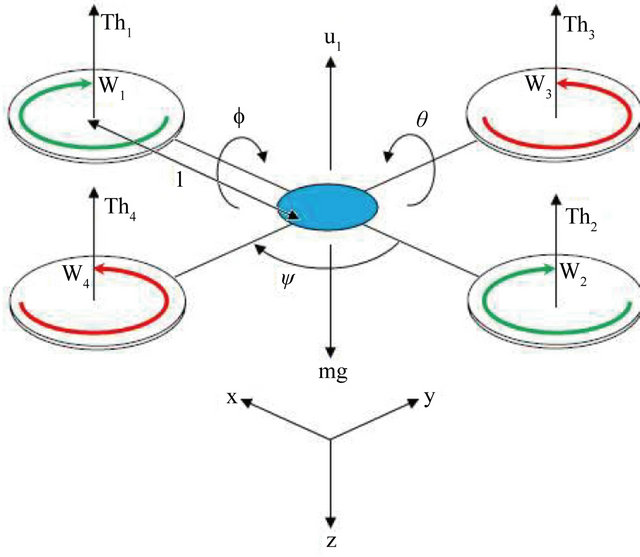
\includegraphics[width=0.70\textwidth]{img/quad_force_diagram.jpg}
\caption{Quadcopter force diagram. Motors and propellors alternate in direction of rotation so that the drone is stable around the vertical axis. The torque generated by each propellor is cancelled by the propellor opposite it \cite{multicopter_dynamics_3}.}
\label{fig:quad_diagram}
\end{figure}\par
\begin{figure}[ht]
\centering
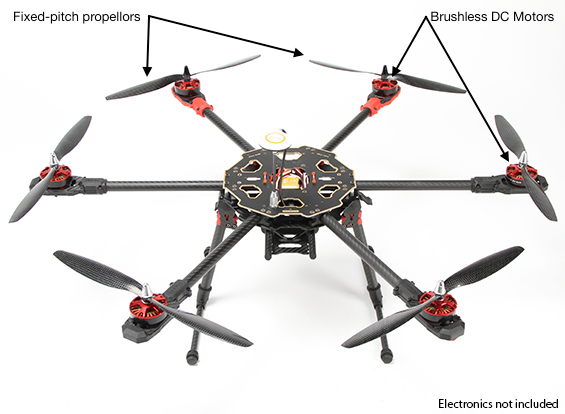
\includegraphics[width=0.70\textwidth]{img/hexacopter.jpg}
\caption{A multicopter with 6 rotors. The brushless DC motors allow for very high speeds and a high degree of control.}
\label{fig:multicopter_hex}
\end{figure}\par
Multicopters use fixed-pitch propellors to correlate rotor speed with force produced. Lift can be controlled by uniformly increasing or decreasing rotor speed across all rotors. To effect a roll or pitch, one side's rotors are spun up and the other side's are spun down so that the net lift remains the same but the craft tilts to the side with less thrust. Multicopters also have the unique ability to yaw in place by spinning alternating rotors faster and slower. Since the rotors alternate in direction of rotation, spinning one set faster creates an imbalance of torque, which makes the whole platform rotate in place \cite{multicopter_dynamics_2}.\par
Multicopters are thus highly maneuverable, but at the cost of flight time and payload capacity. The primary concern when using a multicopter is the flight time. Most commercial multirotors quote flight times in the 10-20 minute range with the best performing drones topping out around 30 minutes \cite{multicopter_comparison}. This is because the power required to spin the electric motors fast enough to get lift can be immense, drawing up to 60 amps on takeoff \cite{multicopter_long_range_mqp}. Ascending from a stationary position draws much more energy than hovering or lateral flying, so multiple takeoffs and landings in one flight will hamper the battery even more. The high current draw of the electric motors necessitates the use of Lithium Polymer (LiPo) batteries that can discharge large amounts of power very quickly. LiPo batteries have another benefit for use in multicopters and that is their low weight.\par
Weight is a very important factor in the operation of a multicopter because the amount of weight to be lifted directly corresponds to the speed the motors must be driven at to achieve lift. Multicopters in general have low payload capacities because any extra weight equates to more power that must be provided by the rotors. In effect, the more weight the drone is carrying, the less flight time it will have. This correlation forces a choice to be made over whether to prioritize flight time or amount of payload supported.\par
The most advantageous aspect of multicopters is their maneuverability. The nature of their control means it is possible to stop and start, hover in place, rotate in place, and quickly change directions and altitudes. In particular, the ability to stop at a point and rotate at a fixed rate is especially unique. To rotate in place, the multicopter increases the speed of all rotors spinning one direction and decreases speed of the other rotors such that the overall lift stays constant, but the torque changes, forcing the whole platform to yaw \cite{multicopter_dynamics}. Deployment of a multicopter is very fast as well: there is nothing that needs assembly prior to flight, and there is no need to find a long open space to takeoff. All that is required procedurally  is powering on the device and setting it on the ground, as multicopters are capable of vertical takeoff and landing (VTOL). The high maneuverability and ease of deployment make for an easy user experience, since control of a drone (with good software) is simple and very responsive. All things considered, the multicopter is a platform that has very good maneuverability, but must sacrifice payload capacity and flight time.
\begin{table}[ht]
\centering
\caption{Multicopter Pros and Cons}
\label{table:multi_pc}
\begin{tabular}{l|l}
  Pros & Cons \\ \hline
  maneuverability & flight time \\
  deployment time & cost \\
   & payload capacity \\
\end{tabular}
\end{table}\par

\section{Chapter Summary}
In this chapter, background information was provided on a range of topics relevant to the undertaken project. The wireless spectrum, divided up into chunks by use, will be the medium for the analysis carried out in this project. Spectrum sensing and localization will be key to achieving the goals of the project. Software Defined Radios are useful for their flexibility around sample processing. Finally, of the flight platforms discussed, multicopters are the only ones with high maneuverability, although they sacrifice flight time and payload capacity to achieve it. This information will allow the informed discussion of implementation of the system for this project.

	\chapter{Proposed Approach}
This chapter will outline the approaches considered to accomplish this project. The goal of this project was to develop a modular platform for sensing the wireless spectrum through the use of a software defined radio (SDR) from an aerial platform. The aerial platform chosen is the multicopter drone due to its controllability and maneuverability. \par

Before proposing the different approaches, it is also important to note that some aspects of this project were fixed by the project’s corporate sponsor. The fixed aspects are as follows: the target spectrum for the project was 2.4 GHz, the software defined radio was the USRP B-200 Mini, and the antenna was the Alfa APA-M25. The software defined radio and antenna were donated to the project by the sponsor Gryphon Sensors. The B-200 Mini was the SDR and the APA-M25 was the antenna. The B-200 Mini has a small form factor or 83.3 x 50.8 x 8.4 mm, has a frequency range of 70MHz to 6GHz, is powered by USB (5V), and has an extensive set of libraries. It is an excellent choice for the spectrum sensing platform primarily due to its frequency range and small form factor. The antenna is designed to be used at 2.4 and and 5GHz, which are the two frequencies WiFi is transmitted at. The antenna is directional with a 16 degree vertical angle and a 66 degree horizontal angle. The high directionality will allow for more accurate determination of the source of the WiFi signal.

% \section{Aerial Platform Selection}
% There were multiple different options regarding what aerial platform would be the best option for the spectrum sensing. These options: kites, fixed wing drones, and multicopters will be discussed in this section. 

% Kites were considered due to their lack of needing an onboard power supply to stay in the air which allows them to stay in the air indefinitely and have a high payload capacity in favorable conditions (constant wind). Since it is not guaranteed that there will be wind in the area where the sensing is needed, the reliability of kites are very low. Kites also have limited mobility, especially in cities where there are tightly packed buildings and other structures, such as street lights that would interfere with the tether to the kite. These drawbacks made the kite unfavorable for use as the aerial platform.

% Fixed wing aircraft were the next option considered. Fixed wing aircraft are able to carry large payloads and fly for extended periods of time, up to multiple hours for gas powered aircraft. Due to a fixed wing aircraft's need for excellent aerodynamics and weight distribution, the payload would have to be created in such a way that it is aerodynamic or can fit in the body of the aircraft, and has to have its weight distributed as to not upset the balance of the aircraft. Although fixed wing aircraft are ideal for open areas, they are almost impossible to use in an urban setting. Most fixed wing aircraft require a long flat runway to takeoff and landing, which limits where they can launch from. They also have a large turning radius that makes it unfeasible for flight in an urban area. Although a fixed wing aircraft has a long flight time and a good payload, its lack of mobility in urban areas makes this unfeasible for the project.

% Multicopters were the final design option considered. Multicopters have a short flight time with the average flight time being between 10-20 minutes. They also have a relatively low payload ranging from a few hundred ounces to a few pounds. Although there are multicopters with high payloads, these aircraft are multiple thousands of dollars. The weight of the spectrum sensing payload would be minimized for use on the cheaper commercial drones. The most attractive quality of the multicopter is its maneuverability. They are able to fly in most any direction and can easily handle flight in cities. Even with the weight requirement and limited flight time, the multicopter is the best option for flight in urban environments. Selection of a multicopter is done in the next section.

\section{Drone Approaches}
For the approach, a multicopter was chosen to be the aerial platform as described in the previous chapter due to the increased maneuverability provided. The maneuverability will allow the platform to perform well in any target environment chosen for spectrum sensing. However, with the drone’s maneuverability, it sacrifices vital airtime and payload capacity, affecting design constraints that will be considered for each of the following approaches. The brainstorming process lead to four distinct design concepts that utilized a multicopter for spectrum sensing. \par

It should be noted that these four designs incorporate similar devices for the single board computer, storage, battery and GPS. Regardless of which drone approach was taken, an onboard processor and storage device had to be chosen for the processing and storage of IQ data. The single board was selected from five options which are shown in Appendix \ref{table:sbc_selection}. The final decision was to use the UP board. The decision was primarily between the UP board and the ODROID-XU4. Both of these boards have a similar form factor, but the UP board draws 1A less current. This reduces the power consumption of the board considerably and negates the lower weight of the XU4. An additional reason for choosing the UP board was the shipping location. The UP board was shipped from Europe, while the Xu4 was shipped from Korea. Therefore, the lead time for the UP board would be shorter and documentation more accessible. As for storage, the selected device was a 32GB usb flash drive, which is capable of storing all the data gathered in one flight simulation of 20 minutes. %10/12/16 MHLI: May need more about other boards.
The external GPS and the battery were chosen for their small form factor. The GPS chosen was the GlobalSat ND-105C micro USB GPS receiver which has a form factor of 30.4mm x 15.4mm x 4.5mm. The battery chosen was the Lumenier 800mAh 3s 20c Lipo Battery which had a form factor of 55mm x 31mm x 20mm.

\subsection{Approach One}
The first approach concept is based upon having an individual wireless communications frequency for each task. Initially this designed was centered around the Autel X-Star that was controlled at 5.7 GHz band. However, upon learning that the 3DR Solo was configurable to operate at 5.7 GHz, and how well the 3DR Solo is documented, the project was then centered around the 3DR Solo. The 3DR Solo is a drone designed as a consumer drone used for aerial photography. The camera and gimbal were replaced with the modular spectrum sensing system to better utilize the limited payload capacity of this drone. The low payload capacity is a good representative of general drones for mounting the modular system, as most consumer based drones are not intended to carry heavy payloads. This drone has a payload capacity of 700 grams, which allows for a substantial payload. While the drone has a large payload capacity, the design will attempt to minimize the payload weight and enable the platform to be used on a larger number of drones. Furthermore, this drone can be configured to operate with the controller at 5.7 GHz that does not interfere with spectrum sensing at the 2.4 GHz wireless band. The transmissions back to the user would be on a frequency of 900 Mhz if real time response is required \cite{3dr_Website}. More detailed design configurations on the first approach can be found in Appendix \ref{table:approach_one}.

\subsection{Approach Two}
The second approach concept is focused on assuring that this project is feasible. This assurance is from the fact that the DJI S1000 octocopter was designed to carry heavier payloads. The DJI S1000 was conceptualized for professional photography and cinematography, where stabilization and high payload is essential as part of the design. Because of these qualities, this drone is priced higher than many consumer-level drones. This drone is able to carry payloads of up to 2 kilograms, providing large flexibility in terms of design constraints. However, because of the flexibility this high payload offers us, the resulting design may not be able to be used on consumer drones with a lower payload capacity. Another advantage this drone presents is that the communication between the controller and the drone is operated at 900 MHz, which will leave the detection of the 2.4 GHz wireless band unimpaired. As for implementation, this drone would serve better as a backup plan in case our modular system can not be lifted with the commercial drones used in testing. More detailed design configurations on the second approach can be found in Appendix \ref{table:approach_two}.

\subsection{Approach Three}
The third approach is based on using an autonomous navigation approach that was considered with the 3DR Solo drone. One of the features that was provided with the drone is autonomous flight planning, where the user can set waypoints for the drone to fly. This feature will allow simplistic controls, however, general drones do not have this feature implemented. Furthermore, the 3DR Solo drone’s ability to be customized is valued, as the initial controller-to-drone transmission frequency is in the target sensing frequency of 2.4 GHz. The autonomy of this design eliminates the need for constant communications with the drone while flying, preventing the control signals from interfering with the spectrum. More detailed design configurations on the third approach can be found in Appendix \ref{table:approach_three}.

\subsection{Approach Four}
The fourth approach concept is focused on shielding the drone’s control antenna from the spectrum sensing antenna. This configuration was created to ensure that the wireless control signals received on the drone and the wireless spectrum being detected would not interfere with each other, since they are on the same frequency. Therefore, a drone carrying 2 antenna configurations would be needed- one that would communicate with the ground, and the other that would perform spectrum sensing. The antennas would need to be isolated from each other in order to ensure the 2 antenna configuration works. This approach would help us have more resilience in our drone platform and would let us have more flexibility on our communication protocols from the ground to the drone. The primary disadvantage to this approach is the additional weight that the shielding would add to the design. More detailed design configurations on the fourth approach can be found in Appendix \ref{table:approach_four}.

\section{Project Planning}
Microsoft Project was used to plan out our objectives throughout the project. The Gantt chart in Figure \ref{fig:gantt_chart} shows our objectives and progress as of early October. The planning came in three parts which are implementation, testing and writing the report. In the initial stages of implementation, each individual part was done first. When each part works separately, the blocks are then integrated to make sure that the system functions as planned. From then on, the project development moves onto the testing stage, where the system is tested in three scenarios. These scenarios allow ease of debugging if the testing does not go according to plan. First, the SDR is tested to determine whether it can locate a WiFi signal without any movement. Then, before mounting the system on the drone, the system will be moved around to check whether the data correlates to a specific direction of a transmitter when the system is mobile. Finally, when both initial tests work properly, the system will be mounted on the drone and tested while flying. During the process of implementation and testing, the report will be written based on the work done in the implementation and testing stages.
\begin{figure}[ht]
\centering
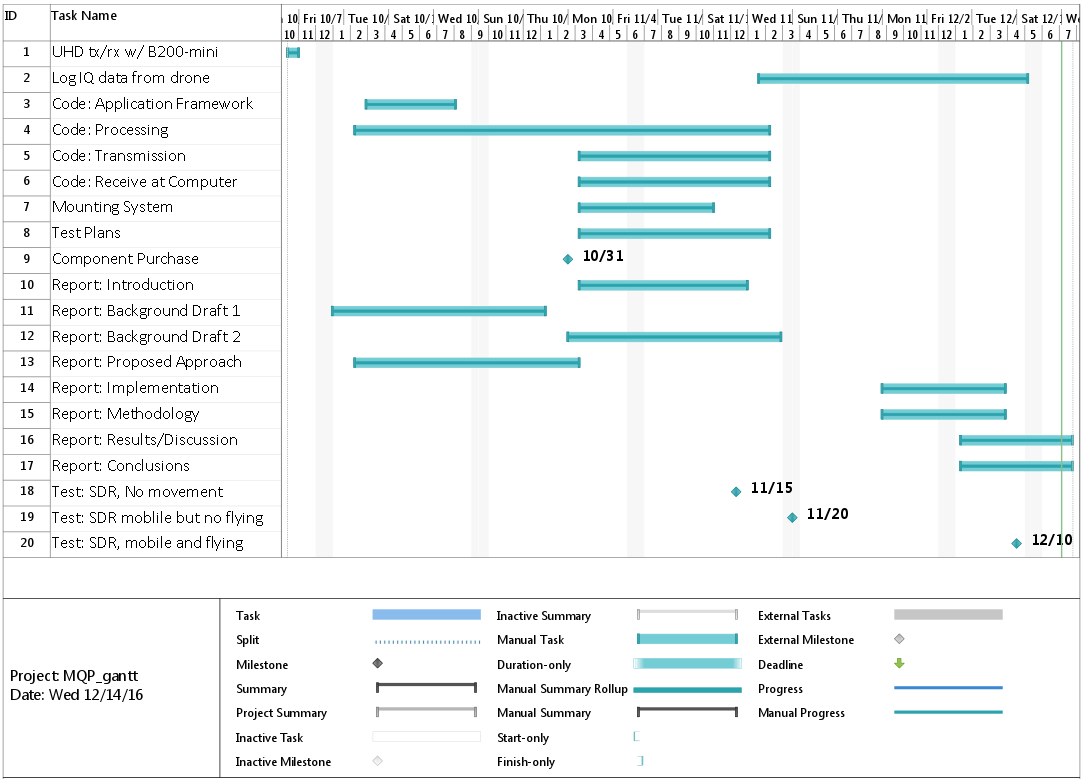
\includegraphics[width=1.0\textwidth]{img/oct_gantt_chart.png}
\caption{Project Planning Gantt Chart}
\label{fig:gantt_chart}
\end{figure}

	
	\chapter{Implementation}

This chapter details the implementation of the MASDR platform. The description has been divided into software and hardware for clarity.

\section{Software Implementation} \label{impl:rotate} \label{impl:tx_messages}
The software for the MASDR system was written in C++ and can be found in Appendix \ref{app:masdr_code}. Documentation was done with doxygen, allowing for dynamic updates to the docs whenever changes were made.  Additionally, some scripts were written to assist in other aspects of the project. \par

%C++ vs gnuradio
During the design phase, there was discussion over whether to use GNU radio or C++ for the MASDR application. GNU radio would allow for more complex signal processing patterns to be constructed more easily in comparison to C++, but would increase the overhead on development and potentially at runtime as well. Using C++, the application would have to be coded entirely from scratch, interfacing with the USRP Hardware Driver (UHD) libraries, but would have much lower overhead. Based on the skills of the team members, as well as the desire for the application to be as low power and simple as possible, C++ was chosen for the application. \par

%Application Structure
The MASDR Application is structured as a central C++ class with a few additional utility functions external to the class. The class contains methods for initialization, sampling, processing, and transmission among others. Certain services, notably updating the GPS and taking in samples, are performed in separate threads to allow for the parallelization of tasks. In the application’s main loop, an instance of the MASDR class updates its status and begins or changes its task based on the new status. Status is composed of both physical status, namely location, and software status, representing the current processing state. The physical status structure includes a member variable for heading, although this is unused in the current version of the platform. The processing state is an enumerated type with values PROCESS, TRANSMIT, and IDLE. The state of the device determines what the processor will be doing. During operation, the application will flow from state to state as described in the state transition diagram in Figure \ref{fig:state_diagram}. \par
\begin{figure}[ht]
\centering
\includegraphics[width=0.70\textwidth]{img/masdr_state_diagram.png}
\caption{MASDR State Diagram. Software states change according to the graph described in the image.}
\label{fig:state_diagram}
\end{figure}
The onboard software is the majority of the project, however there are other essential pieces. On the ground station side, a GNU radio receiver intercepts and decodes all transmissions from the aerial platform. Additionally, a mapping tool was created to calculate the approximate distance to signals and draw circles on a map to visually locate signals. The mapping tool consists of a Python script that performs the distance calculations and populates a Javascript list of GPS locations and distances. The Javascript calls into the Google Maps API to display the distance rings on a map. Finally, a Python script was written to command the drone to autonomously spin 360 degrees. \par
%Sampling procedure 
While the original plan was for the sampling routine to be driven by the motion of the platform, a lack of precision and accuracy in the GPS readings rendered this nearly impossible. Therefore, the SDR was configured to constantly take samples, with control originating from a separate processing thread from the main thread. The use of threads allows for shared data throughout the program, which is used to share the  buffer of samples with the main thread. \par
In order to avoid any shared data bugs, the sampling routine fills a buffer of blocks one at a time, eventually overwriting the oldest block to record each new block. At the beginning of the processing routine, a copy of the most recent half of the sample blocks is made. This makes it impossible for the sampling thread to overwrite a block of samples that the processing thread is using. \par
There is a defined motion pattern that the quadcopter should follow in order achieve correct results. At a constant altitude, the quadcopter should travel to a series of points, stopping and rotating 360 degrees at each point. The constant altitude will allow for more accurate localization of signals based on RSSI distance. \par
%Onboard Processing
The samples taken by the SDR are then processed to extract useful information. Given that the MASDR system is designed to be low power, a delineation between onboard processing and processing at the ground station was created. The UP board’s processor is fairly capable, allowing the initial steps of the signal processing to be done onboard. A more indepth description of the processing done onboard the MASDR platform can be found in Section \ref{methods:processing}. The information is processed as much as possible onboard to reduce the size and duration of the transmissions to the ground station. The initial samples are also stored on a flash drive onboard so that post processing can be done on the raw data. \par
To detect the existence of a signal, an OFDM receiver in the MASDR application looks for beacon signals in the sampled data, block by block. The RSS of a beacon signal is recorded with its corresponding location, the location the drone was at when the block of samples were taken. This mapping is then transmitted down to the ground station for further processing.
%Data Transmission 
The MASDR platform is designed to transmit data between processing blocks of samples. The transmission protocol consists of two types of messages: a header packet, and a data packet. The header packet is the first packet sent after processing the data; it contains a transmission ID, the location of the sampling block, and the number of following data transmissions. The data packet consists of a transmission ID which corresponds to its header packet, a heading, and a signal strength for beacon signals. Again, the heading is unused in the current version of the platform, but a future version could make use of the field.

\section{Hardware Implementation}\label{Mounting}
The hardware for the MASDR system consists of the components used and the mounting system employed to attach it to the drone. Using the 3DR Solo’s development guide as a reference, the mounting system was designed to hold all the components securely to the drone. By using the official mounting points on the drone, the hardware was made as robust and efficient as possible.
%mounting on drone 
In order for the hardware to be mounted properly, the MASDR system was mounted onto the drone platform by using the 3DR Solo’s preexisting hardware mount. To do this, the 3DR Solo developer's guide was used to determine the dimensions of the mounting screws so that the mounting platform was able to be easily screwed onto the 3DR Solo \cite{3dr_devguide}. The mounting system connects to the bottom of the 3DR Solo with four M2 screws that are spaced in a 63mm x 41mm rectangular pattern as seen in Figure \ref{fig:solo_mount}.
\begin{figure}[ht]
\centering
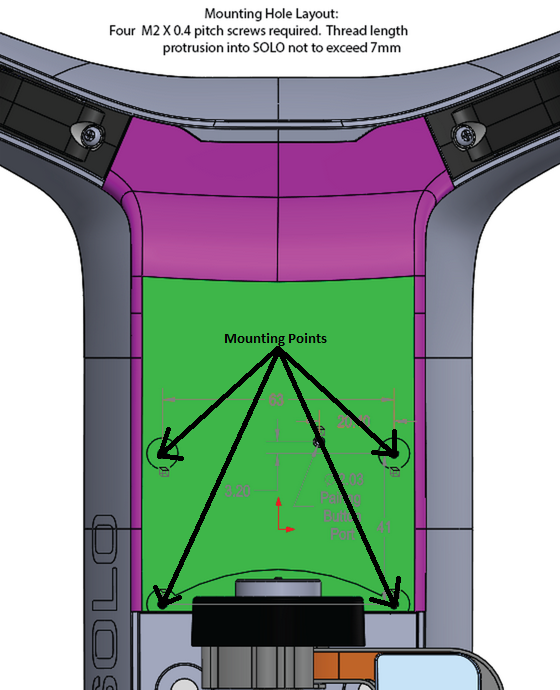
\includegraphics[width=0.70\textwidth]{img/solo_mount_points1.png}
\caption{3DR Solo Mounting Points used for attaching the modular system.}
\label{fig:solo_mount}
\end{figure} \par
The mounting system consisted of two pieces of wood laser cut with and mounting pattern, with unneeded wood removed to reduce weight. The pieces were attached with 3 inch standoffs, allowing room for the UP board, B-200 mini, tranformer, and battery to be mounted and connected together. A picture of the assembled mounting system can be seen in Figure \ref{fig:overhead_of_box} and Figure \ref{fig:box_usb_view}. \par

%Power conversion
In order to ensure that the MASDR platform is powered for the entire flight, a battery was needed that could hold as much energy as possible while not adding too much weight to the drone’s payload. In addition to this, the battery needed be able to supply as much current as the hardware could draw. This became an issue for finding a suitable 5V battery that would support a maximum current draw of 4 Amps. Instead of a 5 volt battery, a 12 volt battery was used, and a DC-DC converter was used to match the 5V 4A requirement. The chosen battery was an 11.1 volt lithium-polymer battery weighing 66 grams. It was then connected to a DROK DC voltage converter that both transformed and regulated the voltage to 5V. By downconverting the voltage from the battery, the system is able to draw more current from the battery than what is usually supported by a 5 volt battery. \par
%Networking card swap
The 3DR Solo’s default wireless card communicates to the controller using the 2.4 GHz band. This interferes with sensing and locating signals on the 2.4 GHz band. In order to avoid this issue, the 2.4 GHz network card of the 3DR Solo was replaced with a dual band 2.4 GHz and 5 GHz network card. Unfortunately, even with the new wireless card, the controller and drone were unable to communicate on the 5 GHz band. It is suspected that this is due to incompatible antennas or configuration scripts on the controller.
 
\section{Implementation Summary}
In this chapter, the implementation of of the MASDR system was detailed from both the software and hardware points of view. The software description covered the application structure, sampling procedures, onboard processing strategy, and data transmission protocol. The hardware section described the mounting system, power conversion, and networking card replacements.The implementation of the system went through multiple iterations during development, and further tweaking and additions to the implementation of the platform are encouraged as needed for any work done using the platform in the future.

 % The application was written in C++ as a central class accompanied by standalone functions to perform tasks such as GPS data aquisition. Sampling is done continuously in its own thread, filling a shared buffer that is later processed and stored to a data file. The onboard processing includes calculating the RSS of the signal and recording the location that the sample was taken. Data transmission is done using a header and data packets for each block of samples. 
 %  The mounting system attaches to the drone using the pre-existing mounting points on the 3DR Solo.  Structurally composed of two wooden panels and large standoffs to create a box, the mounting system held all the components securely together. Power conversion was accomplished with a 12V to 5V DC to DC converter. The wireless cards in the drone and the controller were replaced to allow the drone to be controlled via a 5 GHz signal instead of 2.4 GHz. Although the swap was completed, the communication was still transmitted at 2.4 GHz due to complications. 
	\chapter{Methodology}
\section{Spectrum Sensing} \label{methods:processing}
The main goal of this system is to be able to detect wireless signals. In order to do so, the following sensing methods were used. \hl{Tie together the separate elements - Max}\par
% Energy Detection
The system detects transmissions based off of energy detection. This type of detection is done by measuring our received signal’s strength along a desired central frequency, and comparing it to an ideal threshold. In order to determine the energy of the received signal, the following equation was used:
\[E = \int_{-\infty}^{\infty}| x(t) |^2dt\]
$x(t)$ is the received signal, bandpass filtered to only use the bandwidth of WiFi. This energy measurement is then compared to a threshold energy of -85 dBm. This threshold was chosen due to it being high enough to ensure a low chance of false alarm while still sensing signals from a significant distance, which is necessary since the drone was high in the air. \par

In order to categorize WiFi signals at the 2.4GHz band, an OFDM detector was implemented. In order to detect OFDM, the receiver will detect beacon frames by correlating upon the WiFi’s L-STF structure. The L-STF structure is a specific spacing and timing of transmissions over various subcarriers. This structure is also used for calculating the coarse frequency offset. The subcarriers and transmissions used in L-STF are shown in Figure \ref{fig:ofdm_subcarriers}. \par 
\begin{figure}[ht!]
	\centering
	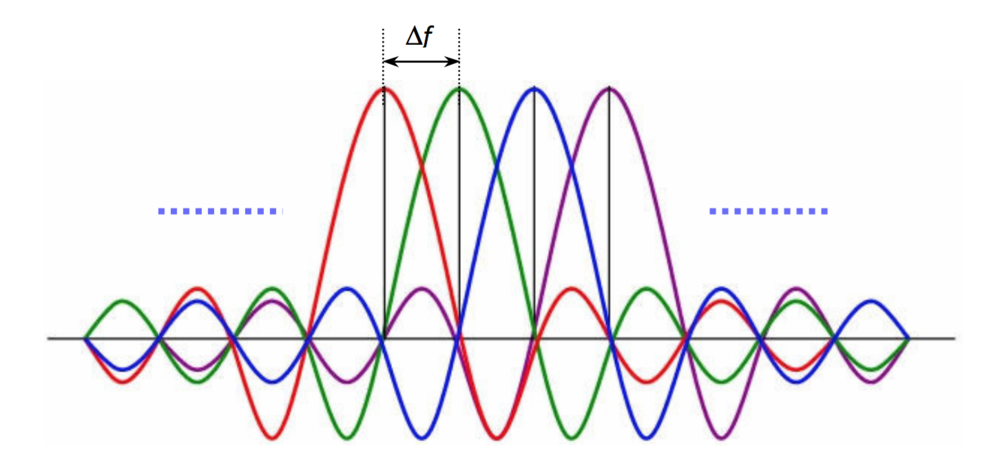
\includegraphics[width=0.70\textwidth]{img/ofdm-subcarriers}
	\caption{This photo gives an example of what OFDM subcarriers look like when displayed upon an FFT.  Each subcarrier is shown as its own respective pulse and the subbcarier frequency offset is denoted by \Delta f.}
	\label{fig:ofdm_subcarriers}
\end{figure}\par
%(https://static1.squarespace.com/static/54860cc3e4b020d690f237ba/t/556cc531e4b0a02f64b72fed/1433191737073/ofdm-subcarriers?format=1000w)
The multiple subcarriers are represented by the various waveform colors in Figure \ref{fig:ofdm_subcarriers}. The spacing of each frequency is denoted by $f$. This series of waveforms are transmitted from the OFDM transmitter over a fixed amount of time. The spacing and frequency behavior of the L-STF field has characteristics defined in Table \ref{table:spacing}: \par
\begin{table}[ht!]
	\centering
	\caption{This table gives an outline on the L-STF Characteristics for an OFDM transmission. Due to our Wi-Fi signals being in the 20, 40, and 80 MHz range, the OFDM match filter will use the values in the first row in order to perform spectrum sensing. The match filter will filter upon a subcarrier spacing of 312.5 kHz by noticing a change in the center frequency of a transmission.}	
\begin{tabular}{|p{3.6cm}|p{4cm}|p{4cm}|p{4.5cm}|}
	\hline
	Channel Bandwidth\newline(MHz) & Subcarrier Frequency Spacing, $\Delta_F$ (kHz) &Fast Fourier Transform Period\newline($T_{FFT}=1/\Delta_F$)& L-STF duration \newline($T_{SHORT}=10*T_{FFT}/4$) \\
	\hline
	20,40,80,160 & 312.5 &3.2$\mu s$ &8 $\mu s$ \\
	10 & 156.25 &$6.4\mu s$ &16 $\mu s $\\
	5 & 78.125 &$12.8\mu s$ &32 $\mu s$  \\
	\hline
\end{tabular} 

	\label{table:spacing}
\end{table} \par 
	
Once a beacon transmission is detected using the above techniques, the L-SIG field must be decoded. The rate field gives us information such as the modulation, coding rate, and data rate by relating the rate to its respective binary value. This field is described in the table below.

%\hl{This table isn't used at all (currently commented out). Do we still need it? If we do we need to talk about it - Max No we do not, it was out of place I think i organized it fine now.}
% \begin{table}[ht!]
% 	\centering
% 	\caption{Details about Various WiFi Transmission Techniques.}
% 	\begin{tabular}{|c|c|c|c|}
% 		\hline
% 		802.11 version & Transmission Vector Format & Modulation Format & Bandiwdths(MHz) \\
% 		\hline
% 		802.11b & non-HT & DSSS/CCK  & 11 \\
% 		802.11a & non-HT & OFDM only & 5,10,20 \\
% 		802.11j & non-HT & OFDM only & 10 \\
% 		802.11p & non-HT & OFDM only & 5,10 \\
% 		802.11g & non-HT & OFDM      & 20 \\
% 			    & non-HT & DSSS/CCK  & 11 \\
% 		802.11n & HT\_MF,non-HT & OFDM only & 20,40 \\
% 		802.11ac & VHT,HT\_MF,non-HT & OFDM only & 20,40,80,160 \\
% 		802.11ah & s1G & OFDM only & 1,2,4,8,16 \\
% 		\hline
% 	\end{tabular}
% 	\label{table:WiFi_table}
% \end{table} \par

\begin{table}[ht!]
	\centering
		\caption{This table gives the corresponding modulation, coding rate, and data rate based on the received binary information from the L-STG field. These fields can then be used to further demodulate the received signal.}
	\begin{tabular}{|l|l|l|l|l|}
		\hline
		Rate(bits 0-3) & Modulation & Coding Rate (R) & 20 MHz data rate (Mb/s) & \\
		\hline
		1101 & Modulation & BPSK & 1/2 & 6 \\
		1111 & Modulation & BPSK & 3/4 & 9 \\
		0101 & Modulation & QPSK & 1/2 & 12 \\
		0111 & Modulation & QPSK & 3/4 & 18 \\
		1001 & Modulation & 16-QAM & 1/2 & 24 \\
		1011 & Modulation & 16-QAM & 3/4 & 36 \\
		0001 & Modulation & 64-QAM & 2/3 & 48 \\
		0011 & Modulation & 64-QAM & 3/4 & 54 \\						
		\hline
	\end{tabular}
	\label{table:ofdm_rate_table}
\end{table} \par

By the rate information, the received packet's 802.11 frame can be further analyzed to find the broadcast SSID of our received transmission frame. The SSID field which starts at the $36^{th}$ byte of the beacon frame header is the only desired information here as it allows the identification of separate access points.
\begin{figure}[ht!]
	\centering
	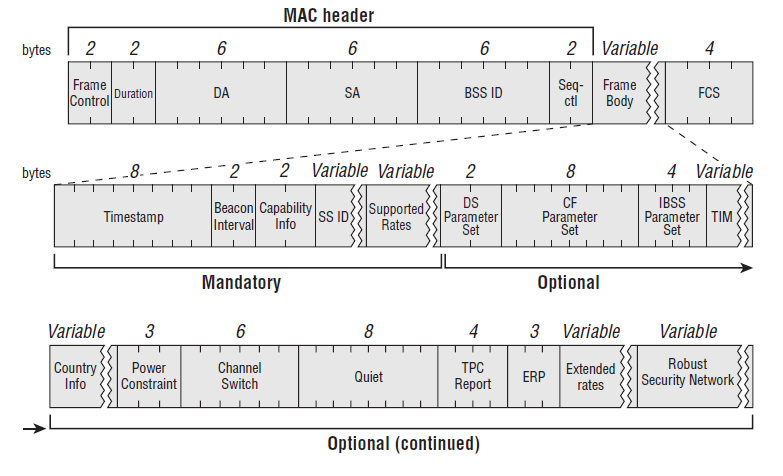
\includegraphics[width=0.70\textwidth]{img/beacon_frame}
	\caption{Beacon Frame Structure \hl{Elaborate and cite source - Max}}
	\label{fig:beacon_frame}
\end{figure}\par
By converting these bits to ASCII, the SSID of the received transmission can be obtained. \par

%Summary
Using a combination of energy detection and match filtering on OFDM beacon frames, the MASDR system was able to identify the desired signals with a high probability of detection and a low probability of false alarm. Additionally, this makes accurate determination of the received SSID possible.

\section{Fusion and Localization} \label{methods:kf}
In order to draw meaning from the spectrum being measured, two types of data need to be analyzed: received signal strength (RSS) and location. Both of these measurements have noise to some extent. In this section, the combination of these measurements and the mitigation of sensor noise was discussed. \par  

%RSS and Direction Readings
After identifying a signal, the next step is to locate the signal source. Out of the methods described in the background, most are ruled out based on the non-cooperative nature of the sensing, leaving only Angle of Arrival (AoA) and RSS localization. Of those two methods, Angle of Arrival is the significantly more complex method to implement, requiring either a strongly directional antenna or an array of antennas \cite{local_aoa}. As such, RSS localization was the method implemented. This method requires three stationary observation points, as opposed to the single moving observation point contained on the aerial platform. To get around this requirement, it is assumed that the device broadcasting the WiFi is stationary \cite{rss_calc}. This assumption is valid because most access points are indeed stationary and the drone moves quickly enough that even a slowly moving signal would likely be able to be roughly located.\hl{Put Diagram of This situation here - Max} \par 
Occasionally while sampling, the drone will rotate continuously in a process described in Section \ref{impl:rotate}. This presents a complication to the processing of the signal: only one sample is recorded at a given angle. Since the samples must be processed in blocks, each block will represent samples from a range of angles. Since the heading measurement is not implemented in the current version of the system, this is of little concern, but for future use, the scenario has been analyzed. \par
The angles included in a block are determined by the amount the drone rotates between the first sample and the last sample of the block. In a small enough block, the error generated by the difference in direction is minimal. However, a smaller block represents a smaller amount of time, in which the signal is more prone to being affected by noise. One solution is to slow down the angular velocity of the drone. While this can be done, the resulting design would be less modular, depending more heavily on the programmability of the drone in use. The other solution is to increase the block size, increasing the amount of time measured, but introducing the problem of deciding what direction should correspond with the resulting signal measurement. Regardless of how this is chosen, the larger block size increases the error in the localization measurement.\par 

In a magnetometer-enabled version of the system, a block size of 131,072 should be chosen. The 3DR Solo rotates at around 2 seconds per rotation. This means that it takes roughly 0.0222 seconds to rotate 4 degrees. At a sample rate of 5 MSPS, this is 111,111 samples. In order to input the signal into the FFT, the block size has to be a power of 2. The nearest power of 2 is $2^{17}$, which is 131072. Each block consists of the second half of the previous block and the next half block of samples. The first block has no previous block, so is just the first 16384 samples. The processed measurement is associated with the direction in the middle of the angle sweep covered by the block. This method introduces a maximum of one degree of error, which is on the same order of magnitude as the error in the HMC5883L magnetometer, a common chip \cite{magnetometer_data}. \par 
The shifting nature of wireless channels introduces a difficult to predict noise into the measurements taken. In order to mitigate this, the drone can rotate multiple times. The resulting received signal strength measurements can then be averaged with the readings from each rotation. This averaging reduces the chance that a random shift in the channel will negatively impact the direction readings. \par 
%GPS
The MASDR system uses GPS readings for location. The distance of the beacon from the drone at multiple points is then used to get an estimated location of the beacon. Within a GPS receiver, signal correction is often carried out. This results in a cleaner and usually more accurate measurement. In addition to this, the receiver that is used in this project polls much less frequently than the localization technique, at around 10 times a second. Since this is higher frequency than is needed, the readings are put through a Kalman Filter to increase the location accuracy. \hl{Add more details on this -Max}\par 
%Kalman Filtering
The GPS receiver that is used in this project provides very noisy results, providing at best 25 meter accuracy when tested in one location. A contributing factor to this is that the receiver used is both small and cheap. Consequently, the values that it reads are frequently very scattered, with a high variance. In order to mitigate this, a four-state Kalman Filter was designed and simulated in MATLAB. The Kalman Filter equations presented in the Chapter \ref{Background} are reproduced below \cite{kf_book}: \par
\subsubsection*{Predict:}
\begin{align}
    \vec{x} &= \matr{F}\vec{x} + \matr{H}\vec{u} \label{eq:state_predict}\\ 
    \matr{P} &= \matr{F}\matr{P}\matr{F^T} + \matr{Q} \label{eq:var_predict}
\end{align}
\subsubsection*{Update:}
\begin{align}
    \vec{y} &= \vec{M} - \matr{H}\vec{x} \label{eq:innovation_up}\\
    \matr{S}&= \matr{HPH^T+RS} \label{eq:inter_up}\\
    \matr{K} &= \matr{PH^TS^{-1}K} \label{eq:kalgain_up}\\
    \vec{x} &= \vec{x} + \matr{K}\vec{y} \label{eq:state_up}\\
    \matr{P} &= \matr{(I-KH)P} \label{eq:var_up}
\end{align} \par
The state $\vec{x}$ holds the $x$ position, $y$ position, $x$ velocity and $y$ velocity. \\
\begin{align}
	\vec{x} &= \begin{bmatrix}
				d_x \\
				d_y\\
				v_x\\
				v_y
				\end{bmatrix}
\end{align}\par
Since we are just estimating the GPS measurement, there is no input that adjusts the values, so $\vec{u} = 0$. The state transition matrix $\matr{F}$ is based on how elements of the states interact with each other. In order to ensure that the filter isn't too complex, a constant velocity model is used \cite{kf_book}. With a small enough $dt$, this is a valid assumption. Because velocity is the derivative of position, $\matr{F}$ is defined as follows: 
\begin{align}
	\matr{F} &= \begin{bmatrix}
					1 & 0 & dt & 0 \\
					0 & 1 & 0 & dt \\
					0 & 0 & 1 & 0 \\
					0 & 0 & 0 & 1
				\end{bmatrix}
\end{align} \par
$\matr{P}$ is the variance matrix for the state, and is initialized as a diagonal matrix with the variance of each individual element. While the assumption that position and velocity are independent is oversimplified and na{\"i}ve. However, since $\matr{P}$ gets updated, this assumption is acceptable. 
$\vec{y}$ is the difference between the most recent measured value $\vec{M}$ and $\matr{H}\vec{x}$. H is set as an identity matrix, so $\vec{y}$ ends up being the difference between a measurement and its prediction. 
Both $\matr{Q}$ and $\matr{R}$ are noise covariance matrices; $\matr{Q}$ is the environment noise covariance, and $\matr{R}$ is the model noise covariance. In order to avoid complications, both of these are assumed to be piecewise white noise. this produces the matrix: 

\begin{align}
Var_v * \begin{bmatrix}\frac{dt^4}{4} & 0 & \frac{dt^3}{2} & 0\\0 & \frac{dt^4}{4} & 0 & \frac{dt^3}{2}\\\frac{dt^3}{2} & 0 & dt^2 & 0 \\ 0 & \frac{dt^3}{2} & 0 & dt^2  \end{bmatrix}
\end{align} \\
The variance is chosen to best fit the data. \par
$\matr{K}$ is the Kalman gain of the system. With a constant noise and variance, this matrix is constant. This is beneficial, as the matrix inverse (or pseudo inverse) that is needed to compute $\matr{K}$. In this implementation, the MATLAB simulation will approximate $\matr{K}$, and the resulting values was used. \par
Equations (\ref{eq:state_up}) and (\ref{eq:var_up}) are used to update the state and state covariance with the most recent measurement.\par

%summary
Both of the two measured values play a role in the localization of a beacon. The GPS location provides a base location from which to reason about the location of the beacon. This location is produced from a Kalman filter, reducing the variance of the measurements. Then, using the RSS measurement of the signal, a ring of possible locations is found around the GPS location. Eventually, measurements from multiple points are used together to get an accurate location of the beacon. Both of these values also have some noise inherent to the process that they are measuring. By taking multiple measurements and calculating the intersections of the rings to signals, the accuracy of the localization is improved.

\section{Drone Control and Communications}
When dealing with multiple frequencies, interference is an issue that must be considered. Interference in the scope of this project may lead to interruptions to drone control, faulty measurement of data, and faulty transmission of data. To help solve these issues, the following steps were taken in drone control and drone communications.\par 

%Drone Control
With the choice of using remote controlled drones to sense WiFi signals comes the problem of interference between the control signal and the WiFi being searched for. This problem is relevant with the use of the 3DR Solo, as the chosen WiFi detection frequency is 2.4 GHz and the 3DR Solo’s operating frequency is also at 2.4 GHz. To alleviate the possible skew of data that the control signal may cause, the 2.4 GHz wireless card of the drone and the controller was changed to a dual band card that supports the 5.7 GHz band. Real time data transmission from the aerial platform to the ground station uses the 900 MHz band. Between the two additional bands used, the 5.7 GHz band was chosen to be the control frequency because of its shorter range due to higher frequencies losing energy faster. The logic behind the decision is that if the drone cannot be controlled properly, then the data obtained from the transmission would not be of significance. Furthermore if the control frequency was 900 MHz, then the drone would be controllable farther away than it would be able to transmit data back to the user, which is not a useful feature.\par 
With the popularity of the 3DR Solo and its ability to be customized, an online discussion board was created for 3DR Solo users to share their experiences with other fellow users \hl{Put ref to board here - Max}. This discussion board provides relevant information on the capabilities and drivers of this commercial drone and customizations that different users have tried. In one thread, a user significantly improved the controls communication range of the drone by swapping the 2.4 GHz wireless card to a higher powered one. This example was the basis of changing the wireless card from 2.4 GHz to 5.7 GHz.\par 
The wireless cards used on the 3DR Solo are mini PCIe and are based on the Atheros AR9382 chip \hl{Put ref here - Max}. Both the controller and the 3DR Solo have these cards for transmission and receiving. The 3DR Solo also uses the ath9k driver that works with a range of Atheros based cards. Based off these requirements, the possible wireless cards that were suitable for replacing the ones on the 3DR Solo were limited. The decision was made to use the MikroTik R11e-5HnD card because it uses the Atheros AR9382 chip that is compatible with the 3DR Solo. As complications arose, detailed in Section \ref{results:drone_ctl}, the SparkLAN WPEA-121N MiniPCI-E Half-Size wireless card was used instead. When physically replacing the wireless card, a YouTube tutorial was used for guidance \hl{Put ref here - Max}. \par 

%Drone Communications
For the drone to send data back to the user, the wireless carrier of 900 MHz was used so that it would not interfere with either the control frequency or the detection frequency. The data packet starts off with multiple consecutive start bits, signaling to the user the beginning of the data transmission. Following the start bits is the data packet itself, of which there are multiple different types, described in Section \ref{impl:tx_messages}. The data inside the packet is interleaved 5 times, meaning that the data will recur at least 5 times to ensure that the data received at the receiver side is consistent. The modulation scheme is DBPSK to increase the quality of the received signal. Additionally, to reinforce the integrity of the signal, the signal is modulated with a root raised cosine (RRC) filter. Furthermore, to avoid corruption of the data packet, a checksum is calculated and appended at the end of the packet. The transmission is concluded by a stream of zeros. \hl{Add state diagram for how comms works - Max}\par

\section{Testing}
For this project, two main categories of test environments were selected for testing the aerial software defined radio: rural and urban areas. The initial testing was in the rural areas, where there are limited interfering wireless signals. The testing was done in a forested backyard so that the SDR was isolated from any interfering communications, providing a good model of using the drone for search and rescue tasks. The path of a signal is shown below in Figure \ref{fig:tree}
\begin{figure}[ht!]
	\centering
	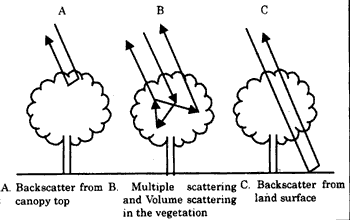
\includegraphics[width=0.70\textwidth]{img/Pathloss_tree}
	\caption{The possible paths of a signal through vegetation. \cite{backscatter}}
	\label{fig:tree}
\end{figure}\par
When testing in urban areas, the drone was used to collect IQ data to map hotspots and eventually locate a specific wireless signal. However, testing in urban areas will require more planning due to air restrictions in cities as the drone can be an issue regarding privacy and possible physical collision. Urban areas are also more likely to have conflicting signals using the 2.4 GHz frequency band. The team will collaborate with Worcester Polytechnic Institute (WPI) to use their parking area in the city, shown below in Figure \ref{fig:gateway} to test out the full system.\par

\begin{figure}[ht!]
	\centering
	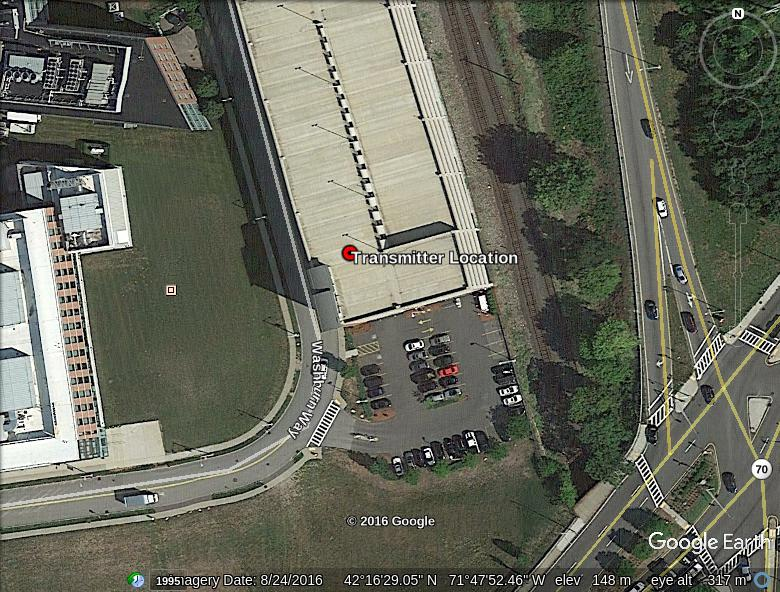
\includegraphics[width=0.70\textwidth]{img/gateway_garage}
	\caption{Location of the Gateway Parking Garage where the urban test was conducted.}
	\label{fig:gateway}
\end{figure}\par

%SDR Operational Test
The first test was to ensure that the SDR is functioning properly. In this test, simple transmitter and receiver code was loaded onto the board. The SDR will then transmit a signal which was acknowledged and logged by a receiver. The receiver will then send out a signal that the SDR will receive and log. The logged signals was observed and compared to the expected result. The test plan is shown below:

\begin{enumerate}
   \item Turn on receiver
   \item Turn on SDR
   \item SDR transmits signal to receiver
   \item Receiver sends acknowledgement to SDR
   \item SDR logs acknowledgement
\end{enumerate}


%Dont think we need a table
%\begin{table}
%\centering
%	\caption{Test environments. \hl{Elaborate, and make table - Max}}	
%\begin{tabular}{|l|l|l|l|}
%	\hline
%\end{tabular} 
%	\label{table:test_env}
%\end{table}
\par 

%SDR Localization Algorithm
The following tests waere conducted using the SDR and a controller as a WiFi transmitter in a parking lot, in a wooded area, and an urban area. The parking lot provided an environment that has a large open space to ensure that the SDR and the WiFi transmitter maintain an unobstructed line of sight. A parking lot with minimal WiFi interference was used to allow for near ideal conditions for preliminary testing. The rural environment provided no interference from other WiFi sources, but provided obstructions in the form of foliage. The urban area provided an environment with both obstructions and non-line-of-sight. This environment was the most challenging to locate the WiFi transmitter in. The following tests were conducted in each of these areas with the SDR not attached to the drone and attached to the drone. When the SDR is attached to the drone, the tests were repeated at different heights, increasing by 30 feet with the maximum height being 150 feet.\par 
The first test will consisted of the SDR being stationary and the WiFi transmitter moving. The test began with the transmitter being placed directly in front of the SDR. The transmitter was moved in a direction, first straight out from the antenna, then to the side of the antenna, and final to the back of the antenna. This was done at a constant speed and the received signal strength was measured over a period of 30 seconds.\par 
The next test was to move the SDR with a stationary transmitter within the line of sight of the SDR. The SDR was moved to different points around the transmitter while measuring the received signal strength. At each point, the SDR stopped and rotated 360 degrees at a steady pace with the rotation lasting approximately two and a half seconds. In the urban and rural environments, this test was also run with the transmitter out of the line of sight of the SDR. In the rural area, this was behind a tree and for the urban area behind a car or building. These tests was performed multiple times and the data was analyzed to determine whether the drone was able to locate the transmitter. The test steps are shown below: \par 

\begin{enumerate}
   \item Position transmitter in a known location (in or out of LOS)
   \item Turn on drone and controller
   \item Fly drone to the testing altitutde
   \item Fly drone in a grid pattern
   \item Approximately every 20 feet rotate the drone 360 degrees at a constant speed for 2.5 seconds
   \item Repeat step 5 until grid pattern is complete
\end{enumerate} \par

%Testing summary
These tests verified that the system is working correctly. Each test increases in complexity and exercised the system to observe its performance in different environments. The first test is simple to verify that the components are working correctly. The second test is done to measure the signal strength at different distances and angles relative to the antenna to be able to evaluate the range at which a transmitter can be detected. The final tests was to localize the signals and distinguish between multiple transmitters.

\section{Summary}
\hl{Put Chapter summary here - Max}

	
	\appendix
\chapter{MATLAB Code}

\section{Energy Detection Example}
\label{app:energy_detection}
\lstinputlisting[basicstyle=\linespread{0.2},language=MATLAB]{../MATLAB_Scripts/energy_detect_masdr.m}
\pagebreak

\section{Matched Filter Example}
\label{app:matched_filter}
\lstinputlisting[basicstyle=\linespread{0.2},language=MATLAB]{../MATLAB_Scripts/matched_filt_masdr.m}
\pagebreak

\section{GPS Kalman Filter Simulation}
\label{app:kf_sim}
\lstinputlisting[basicstyle=\linespread{0.2},language=MATLAB]{../MATLAB_Scripts/Kalman_sim_gps.m}
\pagebreak

\section{Post-Processing Script}
\label{app:matlab_proc}
\lstinputlisting[basicstyle=\linespread{0.2},language=MATLAB]{../MATLAB_Scripts/data_manip_masdr.m}
\pagebreak

\chapter{Python Code}
\chapter{C++ Code}
\section{iq\_to\_file Source Code}\label{app:iq_to_file}
\lstinputlisting[basicstyle=\linespread{0.2},language=C++]{../iq_to_file/iq_to_file.cpp}

\pagebreak
\chapter{Design Configurations}
\section{SBC Selection}
\begin{landscape}
    \begin{table}[h!]
    \caption{SBC Selection}
    \label{table:sbc_selection}
    \centering
    \begin{tabular}{|l|l|l|l|l|l|l|}
        \hline              & ODROID-XU4 & UP Board       & Inforce 6540   & EPIA-P90       & Jetway NP93   & Jetson TK-1      \\ \hline
        Size                & 82 x 58 mm & 86 x 57 mm     &                & 100 x 72 mm    & 100 x 72 mm   &                  \\
        Weight              & 38 grams   & 88 grams       &                &                &               &                  \\
        Power Usage         & 1-4A       & 3A             & 3A             &                &               &                  \\
        Power Voltage       & 5V, 4A     & 5V, 3A         & 12V, 3A        & 12V            &               &                  \\
        CPU                 & Exynos5422 & Intel x5-Z8350 & Snapdragon 805 & VIA Eden       & Intel N2930   & NVIDIA Quad Core \\
        RAM                 & 2GB        & 4GB            & 2GB            & Up to 8GB      & 2GB           & 2GB x 16         \\
        USB 3.0             & Yes        & Yes            & Yes            & Yes            & Yes           & Yes              \\
        OS                  & Linux      & Windows/Linux  &                & Windows/Linux  & Windows/Linux &                  \\
        Price               & \$74       & \$130          & \$240          & \$359          & \$200         & \$192            \\ \hline
    \end{tabular}
    \end{table}
\end{landscape} \par
\section{Approach One}
\begin{table}[h!]
\centering
\caption{Approach One Design Configuration}
\label{table:approach_one}
\begin{tabular}{|l|l|}
    \hline  \textbf{Hardware Design}              & \textbf{Description}                      \\ \hline
            Drone                                 & 3DR Solo                                  \\
            SDR                                   & B-200 Mini                                \\
            Antenna                               & Alfa APA-M25                              \\
            Flight Time                           & 25 min                                    \\
            Flight Speed                          & 5-10 mph                                  \\
            SBC (Computer)                        & Up Board                                  \\
            Compute Battery                       & 12V 800mAh stepped down to 5V             \\
            Payload                               & 700 grams                                 \\
            Storage                               & 32 GB flash drive                         \\
            Antenna Configuration                 & Antenna pointed down                      \\
    \hline  \textbf{Communications Design}        & \textbf{Description}                      \\ \hline
            Drone operation                       & Human Controlled                          \\
            Environment to Drone Frequency        & 2.4 GHz                                   \\
            Controller to Drone TX Frequency      & 5.7 GHz                                   \\
            Controller to Drone TX Period         & Instantaneous (Drone dependent)           \\
            Controller to Drone TX Content        & Control                                   \\
            Drone to Base TX Frequency            & 900 MHz                                   \\
            Drone to Base TX Period               & 2 Hz (Every time drone stops)             \\
            Drone to Base TX Content              & Location and power level if detected      \\
    \hline  \textbf{Signal Processing Design}     & \textbf{Description}                      \\ \hline
            Onboard Computer Processing           & Sensing                                   \\
            Offboard Computer Processing          & Localization                              \\
            SDR FPGA Processing                   & Available if needed                       \\
            Real Time Localization                & No                                        \\
            Sampling Technique                    & User controlled, record bursts of data    \\
            Sampling Space Distance               & User Controlled                           \\
            Number of Samples per Location        & Bursts every half second                  \\
            Localization Method                   & RSS Triangulation (Average RSS over time) \\
            Energy Sensing Technique              & Filter and energy detection               \\ \hline
\end{tabular}
\end{table}\par
\pagebreak
\section{Approach Two}
\begin{table}[h!]
\centering
\caption{Approach Two Design Configuration}
\label{table:approach_two}
\begin{tabular}{|l|l|}
    \hline  \textbf{Hardware Design}              & \textbf{Description}                      \\ \hline
            Drone                                 & DJI S1000                                 \\
            SDR                                   & B-200 Mini                                \\
            Antenna                               & Alfa APA-M25                              \\
            Flight Time                           & 25 min                                    \\
            Flight Speed                          & 5-10 mph                                  \\
            SBC (Computer)                        & Up Board                                  \\
            Compute Battery                       & 12V 800mAh stepped down to 5V             \\
            Payload                               & 2000 grams                                \\
            Storage                               & 32 GB flash drive                         \\
            Antenna Configuration                 & Antenna pointed down                      \\
    \hline  \textbf{Communications Design}        & \textbf{Description}                      \\ \hline
            Drone operation                       & Human Controlled                          \\
            Environment to Drone Frequency        & 2.4 GHz                                   \\
            Controller to Drone TX Frequency      & 900 MHz                                   \\
            Controller to Drone TX Period         & Instantaneous (Drone dependent)           \\
            Controller to Drone TX Content        & Control                                   \\
            Drone to Base TX Frequency            & 5.7 GHz                                   \\
            Drone to Base TX Period               & 2 Hz (Every time drone stops)             \\
            Drone to Base TX Content              & Location and power level if detected      \\
    \hline  \textbf{Signal Processing Design}     & \textbf{Description}                      \\ \hline
            Onboard Computer Processing           & Sensing                                   \\
            Offboard Computer Processing          & Localization                              \\
            SDR FPGA Processing                   & Available if needed                       \\
            Real Time Localization                & No                                        \\
            Sampling Technique                    & User controlled, record bursts of data    \\
            Sampling Space Distance               & User Controlled                           \\
            Number of Samples per Location        & Bursts every half second                  \\
            Localization Method                   & RSS Triangulation (Average RSS over time) \\
            Energy Sensing Technique              & Filter and energy detection               \\ \hline
\end{tabular}
\end{table}\par
\pagebreak
\section{Approach Three}
\begin{table}[h]
\centering
\caption{Approach Three Design Configuration}
\label{table:approach_three}
\begin{tabular}{|l|l|}
    \hline  \textbf{Hardware Design}              & \textbf{Description}                      \\ \hline
            Drone                                 & 3DR Solo                                  \\
            SDR                                   & B-200 Mini                                \\
            Antenna                               & Alfa APA-M25                              \\
            Flight Time                           & 25 min                                    \\
            Flight Speed                          & 5-10 mph                                  \\
            SBC (Computer)                        & Up Board                                  \\
            Compute Battery                       & 12V 800mAh stepped down to 5V             \\
            Payload                               & 700 grams                                 \\
            Storage                               & 32 GB flash drive                         \\
            Antenna Configuration                 & Antenna pointed down                      \\
    \hline  \textbf{Communications Design}        & \textbf{Description}                      \\ \hline
            Drone operation                       & Human Controlled                          \\
            Environment to Drone Frequency        & 2.4 GHz                                   \\
            Controller to Drone TX Frequency      & N/A                                       \\
            Controller to Drone TX Period         & N/A                                       \\
            Controller to Drone TX Content        & Kill/Return home signal                   \\
            Drone to Base TX Frequency            & 900 MHz                                   \\
            Drone to Base TX Period               & 2 Hz (Every time drone stops)             \\
            Drone to Base TX Content              & Location and power level if detected      \\
    \hline  \textbf{Signal Processing Design}     & \textbf{Description}                      \\ \hline
            Onboard Computer Processing           & Sensing, localization, drone control      \\
            Offboard Computer Processing          & None                                      \\
            SDR FPGA Processing                   & Available if needed                       \\
            Real Time Localization                & Yes                                       \\
            Sampling Technique                    & Sample at one spot, move to next spot     \\
            Sampling Space Distance               & User Controlled                           \\
            Number of Samples per Location        & Bursts every half second                  \\
            Localization Method                   & RSS Triangulation (Average RSS over time) \\
            Energy Sensing Technique              & Filter and energy detection               \\ \hline
\end{tabular}
\end{table}\par
\pagebreak
\section{Approach Four}
\begin{table}[h]
\centering
\caption{Approach Four Design Configuration}
\label{table:approach_four}
\begin{tabular}{|l|l|}
    \hline  \textbf{Hardware Design}              & \textbf{Description}                      \\ \hline
            Drone                                 & 3DR Solo                                  \\
            SDR                                   & B-200 Mini                                \\
            Antenna                               & Alfa APA-M25                              \\
            Flight Time                           & 25 min                                    \\
            Flight Speed                          & 5-10 mph                                  \\
            SBC (Computer)                        & Up Board                                  \\
            Compute Battery                       & 12V 800mAh stepped down to 5V             \\
            Payload                               & 700 grams                                 \\
            Storage                               & 32 GB flash drive                         \\
            Antenna Configuration                 & Sheilding around sensing antenna          \\
    \hline  \textbf{Communications Design}        & \textbf{Description}                      \\ \hline
            Drone operation                       & Human Controlled                          \\
            Environment to Drone Frequency        & 2.4 GHz                                   \\
            Controller to Drone TX Frequency      & 2.4 GHz                                   \\
            Controller to Drone TX Period         & Instantaneous (Drone dependent)           \\
            Controller to Drone TX Content        & Control                                   \\
            Drone to Base TX Frequency            & 900 MHz                                   \\
            Drone to Base TX Period               & 2 Hz (Every time drone stops)             \\
            Drone to Base TX Content              & Location and power level if detected      \\
    \hline  \textbf{Signal Processing Design}     & \textbf{Description}                      \\ \hline
            Onboard Computer Processing           & Sensing                                   \\
            Offboard Computer Processing          & Localization                              \\
            SDR FPGA Processing                   & Available if needed                       \\
            Real Time Localization                & No                                        \\
            Sampling Technique                    & User controlled, record bursts of data    \\
            Sampling Space Distance               & User Controlled                           \\
            Number of Samples per Location        & Bursts every half second                  \\
            Localization Method                   & RSS Triangulation (Average RSS over time) \\
            Energy Sensing Technique              & Filter and energy detection               \\ \hline
\end{tabular}
\end{table}\par
\pagebreak


	
	% Bibliography
%	\singlespacing
%	\nocite{*}
%	\bibliographystyle{plain}
%	\bibliography{references}
	
\end{document}









